%% cas-sc-template.tex — FedPOT: Privacy-Preserving Federated Transfer Learning
%% Elsevier CAS single-column format
%% Target journals: Knowledge-Based Systems / Expert Systems with Applications

\documentclass[a4paper,fleqn]{cas-sc}

\usepackage[authoryear,longnamesfirst]{natbib}
\usepackage{algorithm}
\usepackage{algpseudocode}
\usepackage{xspace}
\usepackage{placeins}

%%% Author macros
\def\tsc#1{\csdef{#1}{\textsc{\lowercase{#1}}\xspace}}
\tsc{OT}
\tsc{CVAE}
%%%

%% Theorem-like environments following the Elsevier CAS template.
\newtheorem{theorem}{Theorem}
\newtheorem{proposition}{Proposition}
\newdefinition{definition}{Definition}
\newdefinition{remark}{Remark}
\newproof{pf}{Proof}
\newcommand{\subfigtitle}[1]{%
  {\small\fontfamily{ptm}\selectfont\textbf{#1}}\par\vspace{0.4ex}%
}
\AtBeginEnvironment{table}{\fontfamily{ptm}\selectfont}
\ExplSyntaxOn
\cs_set:Npn \__cas_head:
{
  \parbox{\textwidth}
    {
      \fontfamily{ptm}\selectfont\small\centering
      \__short_title:
    }
}
\cs_set:Npn \__make_tbl_caption:nn #1#2
{
  \skip_vertical:N \l_tbl_abovecap_skip
  \parbox{ \l_tbl_width_dim }
    {\rightskip=0pt\fontfamily{ptm}\selectfont\small
     \textbf{\color{scolor}#1}\par#2\par\vskip4pt}
  \skip_vertical:N \l_tbl_belowcap_skip
}
\cs_set:Npn \__make_fig_caption:nn #1#2
{
  \l_fig_align_tl
  \skip_vertical:N \l_fig_abovecap_skip
  \setbox\cascaptionbox=\hbox{%
     \fontfamily{ptm}\selectfont\small\textbf{\color{scolor}#1:}~#2}
  \ifdim\the\wd\cascaptionbox<\dim_use:N \l_fig_width_dim\relax
  	\parbox{ \l_fig_width_dim }
   		{\unskip\ignorespaces\hfil\fontfamily{ptm}\selectfont\small
       \textbf{\color{scolor}#1:}~#2\hfil\par }
  \else
  	\parbox{ \l_fig_width_dim }
   		{\rightskip=0pt\unskip\ignorespaces\fontfamily{ptm}\selectfont
       \small\textbf{\color{scolor}#1:}~#2\par }
  \fi
  \skip_vertical:N \l_fig_belowcap_skip
}
\ExplSyntaxOff

\begin{document}
\let\WriteBookmarks\relax
\def\floatpagepagefraction{1}
\def\textpagefraction{.001}

\shorttitle{FedPOT for Privacy-Preserving Federated Transfer Learning}
\shortauthors{Zilong Yin}

\title [mode = title]{Privacy-Preserving Federated Transfer Learning via Partial Optimal Transport and Transport-Conditioned Generation}


\author[1]{Zilong Yin}[orcid=0009-0002-7994-2772]
\cormark[1]
\ead{zilong_yin@163.con}
\credit{Conceptualization, Methodology, Software, Formal Analysis,
Writing -- original draft, Writing -- review \& editing}

\affiliation[1]{organization={College of Electronic and Information Engineering,
            Tongji University},
            city={Shanghai},
            postcode={201804},
            country={China}}

\cortext[1]{Corresponding author}

\begin{abstract}
Federated transfer learning (FTL) enables cross-domain knowledge sharing
without transmitting raw data, yet simultaneously faces three interlocking
challenges: enforcing differential privacy on transmitted statistics,
aligning heterogeneous feature spaces across domains, and generating
class-informative complementary features for unlabelled target samples.
Existing methods address these challenges in isolation, leaving their
joint optimisation unexplored.
We propose \textbf{FedPOT}, a five-phase FTL framework that tightly
integrates a Gaussian-mechanism differential privacy (DP) guarantee,
partial optimal transport (OT) alignment, and a transport-conditioned
conditional variational autoencoder (CVAE) into a coherent pipeline.
In Phase~1, source class prototypes are sanitised by a calibrated
Gaussian mechanism before crossing the privacy boundary, providing a
formal $(\varepsilon,\delta)$-DP guarantee.
In Phase~2, a partial Wasserstein plan computed on a within-domain
relational cost matrix discovers semantically consistent cluster-to-class
correspondences that are robust to both distribution shift and DP noise.
In Phase~3, a CVAE decoder conditioned on OT transport conditions
generates $d_s$-dimensional complementary features; an entropic Sinkhorn
regularisation term in the CVAE loss pushes the generated distribution
towards the source prototype manifold, and post-generation smoothing
further reduces generation variance by interpolating between the
stochastic CVAE output and the deterministic OT condition.
Phases~4 and~5 apply uncertainty-aware filtering and a two-stage
late-fusion ensemble.
On two real-world benchmarks---the CWRU rolling-element bearing fault
dataset and the Office-Caltech-10 cross-domain image benchmark---FedPOT
outperforms five competitive baselines.
On CWRU, FedPOT achieves the highest accuracy (71.3\%), macro-F1 (70.8\%),
and macro-AUC (86.9\%).
On Office-Caltech-10, where pseudo-label quality bounds hard-decision
accuracy for all unsupervised federated methods, FedPOT attains the
highest macro-AUC (74.8\%), surpassing the nearest competitor by
0.8 percentage points and the no-transfer baseline by 3.3 pp.
A component-wise ablation confirms that partial OT alignment, OT
regularisation, and soft transport conditioning each contribute positively
on both benchmarks.
\end{abstract}

% Use if graphical abstract is present.
\begin{graphicalabstract}
  \centering
  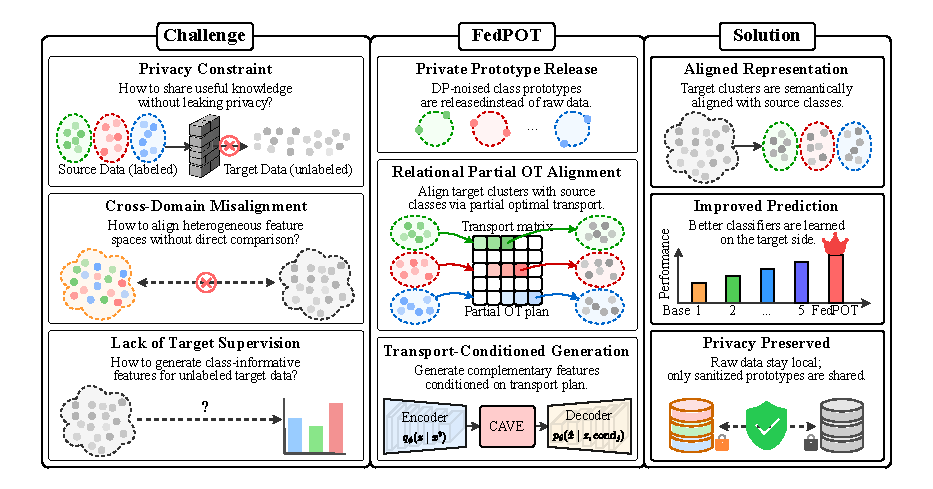
\includegraphics[scale=1.14,trim=20 10 20 11,clip]{figures/Overview.pdf}
\end{graphicalabstract}

\begin{highlights}
\item FedPOT jointly optimises differential privacy, partial optimal
  transport alignment, and conditional generative augmentation in a
  single federated transfer learning pipeline.
\item A relational cost matrix for partial OT enables robust semantic
  alignment under DP noise without direct cross-domain feature comparison.
\item Transport-conditioned CVAE with Sinkhorn OT regularisation and
  post-generation smoothing yields well-calibrated complementary features.
\item FedPOT outperforms five FTL baselines on CWRU (all metrics) and
  Office-Caltech-10 (macro-AUC); ablation confirms all component contributions.
\end{highlights}

\begin{keywords}
Federated transfer learning \sep
Differential privacy \sep
Partial optimal transport \sep
Conditional variational autoencoder \sep
Domain adaptation \sep
Fault diagnosis
\end{keywords}

\maketitle


%%==========================================================================
\section{Introduction}
\label{sec:intro}
%%==========================================================================

Modern intelligent systems increasingly learn from data that are distributed
across institutions, devices, or industrial sites. In healthcare, predictive
maintenance, smart manufacturing, and finance, these parties often describe
related entities through different feature views and are unable to pool raw
records because of privacy, ownership, or regulatory constraints
\citep{Yang2019,Kairouz2021,Rieke2020}. Federated learning (FL) alleviates
part of this tension by replacing raw-data exchange with model or statistic
exchange \citep{McMahan2017,Li2020FedProx,Konecny2016}. However, many
high-value scenarios do not satisfy the standard horizontal FL assumption
that all parties observe the same feature space. A labelled, data-rich source
party may hold one feature view, while a target party holds a different,
unlabelled feature view on a related task. This is the unsupervised
federated transfer learning (FTL) setting considered in this paper.

The difficulty of unsupervised FTL is not merely that data are private or
distributed. Its core difficulty is the coupling of three constraints that
are usually studied separately. First, the source party must communicate
useful transferable knowledge without revealing individual source samples.
Second, the target party must infer how its unlabelled clusters correspond
to source classes, even though source and target features may be
heterogeneous or even disjoint. Third, after such a correspondence is found,
the target party still needs a way to construct class-informative
complementary features that make the transferred knowledge usable by a
downstream predictor. Solving only one of these subproblems is insufficient:
privacy without semantic alignment transmits protected but unusable
statistics; alignment without generation gives only pseudo-labels but no
complementary feature view; generation without privacy-aware alignment risks
producing features that are neither private nor semantically anchored.

Existing methods leave this coupling largely unresolved. Differentially
private optimisation protects gradients but may inject noise into the very
signals needed for cross-domain matching \citep{Abadi2016,McMahan2018DP}.
Adversarial and discrepancy-based adaptation methods can reduce
distributional mismatch, but they typically assume shared feature spaces,
source-model access, or unprotected source representations
\citep{Ganin2016,Long2018,Liang2020}. Prototype-based FL compresses
client knowledge into class representatives, yet prototypes alone do not
identify robust target-to-source correspondences under heterogeneous feature
views \citep{Tan2022Proto,YinCrossKTFRA}. Optimal transport (OT) offers a
principled alignment geometry \citep{Courty2017,Cuturi2013}, but direct
cross-domain distances are unreliable when source and target feature spaces
are not comparable. Conditional generative models can synthesize missing or
complementary views \citep{Kingma2014,Goodfellow2014,Mirza2014}, but they
require a meaningful conditioning signal, which is precisely what
unsupervised FTL lacks.

This paper proposes \textbf{FedPOT}, a privacy-preserving FTL framework that
treats privacy, alignment, and generation as a single design problem. The
source party releases only differentially private class prototypes. The
target party constructs a relational cost matrix from within-domain
distance profiles, uses partial OT to infer a cluster-to-class semantic
bijection, and then conditions a CVAE on the resulting transport signals to
generate source-style complementary features for target samples. An
uncertainty-aware weighting mechanism and a late-fusion classifier turn
these generated features into robust target-side predictions.

\smallskip
\noindent\textbf{Contributions.}
The main contributions are summarised as follows.

\begin{enumerate}
  \item We formulate a privacy-preserving unsupervised vertical FTL pipeline
    in which the only information crossing the source--target boundary is a
    compact set of DP-sanitised source prototypes.

  \item We develop a relational partial OT alignment mechanism that matches
    target clusters to source classes using within-domain structural
    signatures rather than unreliable direct cross-domain distances.

  \item We introduce transport-conditioned generative augmentation, where a
    CVAE is regularised by a Sinkhorn OT term and stabilised by
    post-generation smoothing to produce semantically anchored complementary
    features.

  \item We provide theoretical analysis for privacy, relational alignment
    invariance, generation stability, risk transfer, and communication
    complexity, clarifying why the components are mutually reinforcing.

  \item We conduct a comprehensive empirical evaluation on CWRU and
    Office-Caltech-10, including baseline comparisons, ablations, privacy
    sensitivity, hyperparameter analysis, calibration, communication cost,
    and visual diagnostics.
\end{enumerate}

%%==========================================================================
\section{Related Work}
\label{sec:related}
%%==========================================================================

\subsection{Federated Learning and Federated Transfer Learning}

FedAvg \citep{McMahan2017} established the canonical round-based FL
protocol; subsequent work addressed statistical heterogeneity
\citep{Li2020FedProx,Zhao2018FL,Karimireddy2020}, communication
efficiency \citep{Konecny2016}, Byzantine robustness \citep{Blanchard2017},
and personalisation \citep{Fallah2020,Ghosh2020,Li2021Moon,Yurochkin2019}.
Vertical and federated transfer learning extend the paradigm to
heterogeneous feature spaces \citep{Yang2019,Liu2020FTL,Liu2024}.
Surveys cover system-level \citep{Li2023DPFL} and open-problem
\citep{Kairouz2021} perspectives.
Despite this progress, most FL and FTL methods still rely on at least one of
three assumptions that become restrictive in unsupervised vertical transfer:
model or feature-space compatibility, repeated cross-party optimisation, or
the availability of labelled target-side supervision.
When only a compact privacy-preserving source summary can be transmitted,
these assumptions leave the semantic alignment problem under-specified.

\subsection{Differential Privacy in Federated Learning}

The foundational DP framework \citep{Dwork2014} and the analytically
calibrated Gaussian mechanism \citep{Balle2018} provide the theoretical
basis.
DP-SGD \citep{Abadi2016} clips and perturbs per-example gradients;
client-level DP \citep{Geyer2018,McMahan2018DP} offers stronger
user-level guarantees.
Gradient leakage attacks \citep{Zhu2019} motivate protecting even
summary statistics.
Prototype-level perturbation is communication-efficient because only
$K$ class mean vectors are released, but prototypes remain vulnerable to
semantic distortion when the privacy noise is not explicitly considered by
the downstream alignment module.
\citet{Tan2022Proto} propose prototype synchronisation across heterogeneous
clients but without DP.
Existing DP-FL approaches therefore tend to protect either gradients,
parameters, or simple summaries, yet they rarely analyse how the protected
object can still support reliable transfer under heterogeneous feature
spaces.

\subsection{Optimal Transport for Domain Adaptation}

OT provides a geometry-aware measure of distributional discrepancy
\citep{Villani2008,Peyre2019,Caffarelli2010}.
\citet{Courty2017} used regularised OT for marginal alignment;
\citet{Damodaran2018} (DeepJDOT) integrated OT into deep feature learning;
\citet{Shen2018AAAI} used Wasserstein distance as a representation-learning
objective.
Partial OT \citep{Chapel2020,Chizat2018} relaxes mass conservation,
transporting only a fraction $m$ of total mass, which is critical when
cluster structures differ across domains.
Sinkhorn distances \citep{Cuturi2013} enable efficient, differentiable OT
computation.
Theoretical guarantees on OT convergence appear in \citep{Fournier2015},
and OT generalisation bounds for domain adaptation are established in
\citep{Redko2017,Zhang2019DA,BenDavid2010}.
Wasserstein-based generative objectives \citep{Frogner2015,Genevay2018,
Tolstikhin2017,Alvarez2021} combine OT with neural networks.
However, conventional OT-based adaptation usually presumes directly
comparable feature representations or access to sample-level distributions
from both domains. In vertical FTL, where source and target coordinates are
incompatible and only noisy prototypes are visible, a direct ground cost can
become ill-defined or dominated by privacy-induced perturbations.

\subsection{Generative Augmentation for Transfer Learning}

VAEs \citep{Kingma2014} encode inputs into a structured latent space;
$\beta$-VAE \citep{Higgins2017} promotes disentanglement; Wasserstein
auto-encoders \citep{Tolstikhin2017} replace KL with an OT prior.
GANs \citep{Goodfellow2014} and conditional GANs \citep{Mirza2014} provide
powerful alternatives but are harder to train and require careful mode
coverage.
Sinkhorn divergences \citep{Cuturi2013,Genevay2018} offer differentiable
mini-batch OT objectives suitable for generative regularisation.
Nevertheless, most generative augmentation methods treat generation as a
stand-alone data-expansion step. Without an explicit coupling between the
alignment structure and the generator, synthetic features may improve sample
quantity while drifting away from the cross-domain semantics required for
target discrimination.

\subsection{Source-Free and Source-Hypothesis Transfer}

SHOT \citep{Liang2020} and model adaptation methods \citep{Li2021SFDA}
transfer from a trained source model without raw source features.
The MMD-based distribution matching of \citet{Gretton2012} and adversarial
alignment of \citet{Ganin2016} require direct feature comparison across
domains.
These methods reduce source-data exposure, but they still typically depend on
a source hypothesis, a shared representation, or sample-level distribution
matching. Such requirements are difficult to satisfy when the source party is
allowed to release only a small differentially private prototype set.

%%==========================================================================
\section{Problem Formulation}
\label{sec:problem}
%%==========================================================================

Let $\mathcal{D}_s = \{(x_i^s, y_i^s)\}_{i=1}^{N_s}$ be a labelled
source dataset with $x_i^s \in \mathbb{R}^{d_s}$ and
$y_i^s \in [K] := \{1,\ldots,K\}$.
Let $\mathcal{D}_t = \{x_j^t\}_{j=1}^{N_t}$ be an unlabelled target
dataset with $x_j^t \in \mathbb{R}^{d_t}$.
In the vertical FTL setting, $\mathcal{D}_s$ and $\mathcal{D}_t$ reside on
separate parties that share no raw data.

\begin{figure}[htbp]
\centering
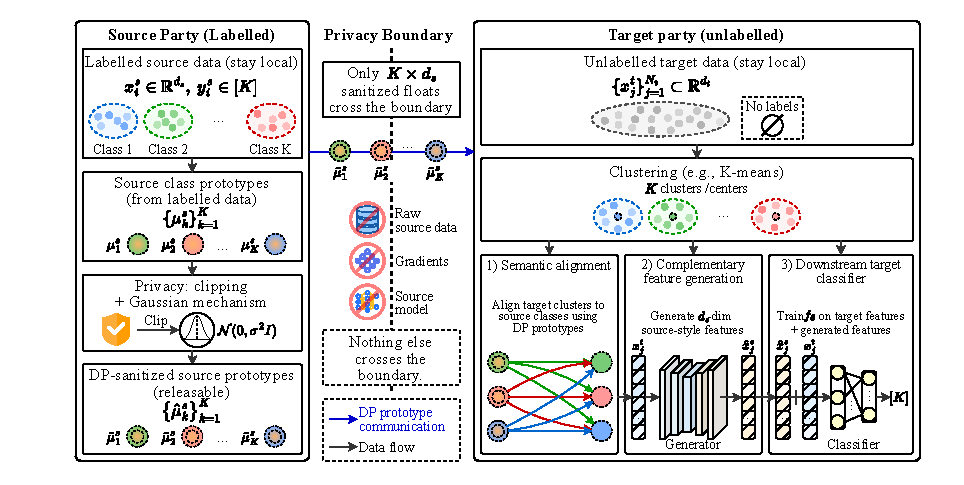
\includegraphics[scale=1,trim=35 10 21 10,clip]{figures/Problem.pdf} 
\caption{\textbf{Problem setting.} The source party owns labelled source-side
    features, the target party owns unlabelled target-side features, and the
    only cross-party information allowed by FedPOT is a small set of
    DP-sanitised source prototypes. The target party must align clusters to
    classes, generate complementary source-style features, and train the
    final classifier without observing raw source samples.}
\label{fig:problem}
\end{figure}

\begin{definition}[Unsupervised Vertical FTL]
  Given $\mathcal{D}_s$ (source, labelled) and $\mathcal{D}_t$ (target,
  unlabelled) on separate parties with no raw-data sharing, learn a
  target classifier $f_\theta: \mathbb{R}^{d_t} \to [K]$ by transmitting
  only $(\varepsilon,\delta)$-differentially private summary statistics from
  source to target.
\end{definition}

The source party transmits DP-protected class prototypes
$\tilde{\mu} = \{\tilde{\mu}_k^s\}_{k=1}^K \subset \mathbb{R}^{d_s}$.
The target party uses $\tilde{\mu}$ to discover cluster-to-class
correspondences, generate $d_s$-dimensional complementary features, and
train a downstream classifier on augmented target-domain data.

\noindent\textbf{Metrics.} We report macro-averaged accuracy (Acc),
macro-F1, and macro-AUC on the target test split.
AUC captures probability calibration quality, critical for risk-sensitive
decision-support scenarios.

%%==========================================================================
\section{The FedPOT Framework}
\label{sec:method}
%%==========================================================================

FedPOT proceeds in five phases, depicted in Fig.~\ref{fig:pipeline}.
The framework is designed around three constraints that jointly distinguish
the considered setting from conventional domain adaptation.
First, the source party must not disclose raw samples, gradients, or a
trainable source model; consequently, the transferable object must be a
compact statistic with an explicit privacy guarantee.
Second, source and target features may live in incompatible coordinate
systems, so cross-domain alignment cannot rely on direct Euclidean or cosine
distances.
Third, the target party is unlabelled, making the generated complementary
features useful only if they preserve the latent cluster-to-class semantics
inferred during alignment.
FedPOT therefore couples the three core operations rather than treating them
as independent modules: DP prototype release defines the only admissible
source information, relational partial OT converts this information into a
semantic transport structure, and the transport-conditioned CVAE uses that
structure as both a generation condition and a distributional regulariser.

\begin{figure}[htbp]
\centering
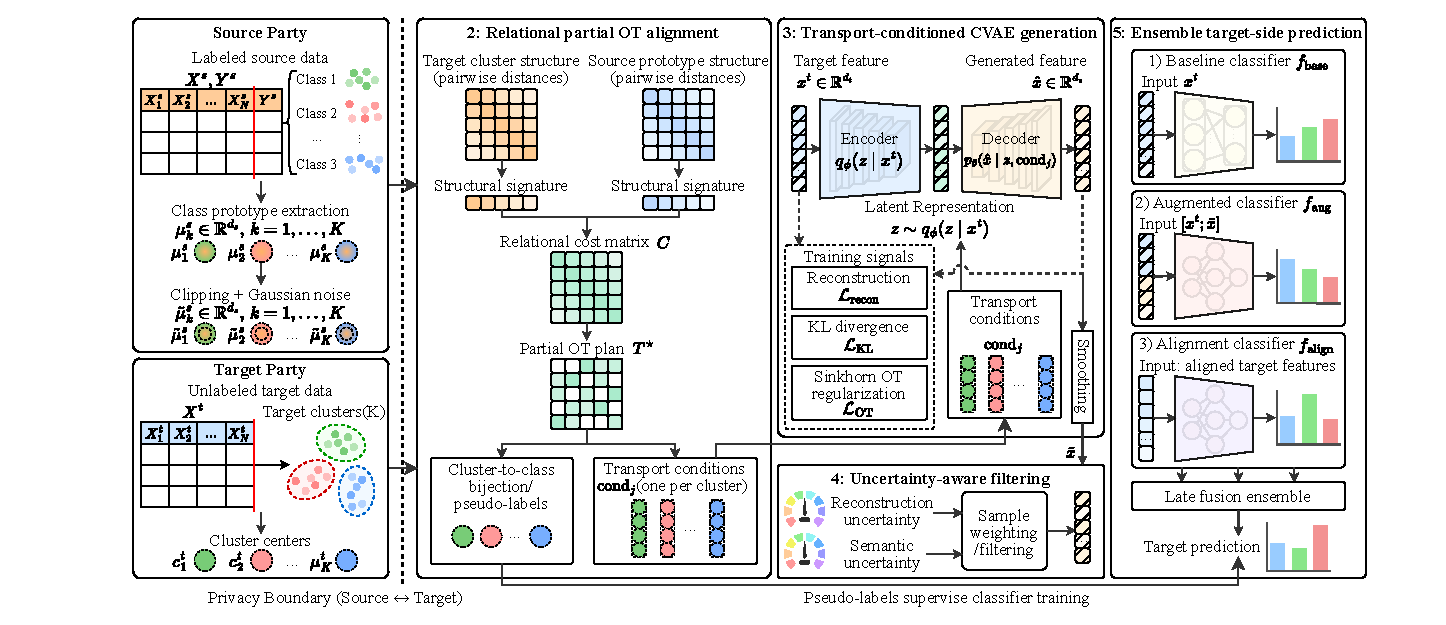
\includegraphics[scale=0.78,trim=63 9 38 8,clip]{figures/FedPOT.pdf} 
\caption{\textbf{Overview of the FedPOT.} All computation except
    Phase~1 source-side prototype extraction is performed on the
    target party. Only $K \times d_s$ sanitised floats cross the
    privacy boundary.}
\label{fig:pipeline}
\end{figure}

%%--------------------------------------------------------------------------
\subsection{Phase 1: Differentially Private Prototype Extraction}
\label{sec:phase1}
%%--------------------------------------------------------------------------

\paragraph{Source-side prototypes.}
The source party computes class-conditional mean vectors:
\begin{equation}
  \mu_k^s = \frac{1}{n_k}\sum_{i:\,y_i^s=k} x_i^s, \quad k \in [K],
  \label{eq:proto}
\end{equation}
where $n_k = |\{i : y_i^s = k\}|$. Individual features are clipped to
$\ell_2$-norm $C_{\max}$ before averaging.
The prototype statistic is deliberately chosen because it preserves the
class-level geometry required for transfer while keeping the privacy
mechanism simple enough to analyse. Compared with sharing a source encoder or
gradient trajectory, the released object has size $K d_s$ and its sensitivity
decreases with the class sample count $n_k$.

\paragraph{Gaussian mechanism.}
Applying the Gaussian mechanism of \citet{Balle2018}, each prototype
is perturbed as
\begin{equation}
  \tilde{\mu}_k^s = \mu_k^s + \xi_k, \quad
  \xi_k \sim \mathcal{N}\!\left(0,\,\sigma_{\rm dp}^2\, I_{d_s}\right),
  \label{eq:dp}
\end{equation}
where
$\sigma_{\rm dp} = C_{\max}\,\sqrt{2\ln(1.25/\delta)}\,/\,(n_k\,\varepsilon)$
is calibrated to the $\ell_2$-sensitivity $C_{\max}/n_k$ of $\mu_k^s$.

\begin{theorem}[DP guarantee, \citealt{Dwork2014,Balle2018}]
  Releasing $\{\tilde{\mu}_k^s\}_{k=1}^K$ under the Gaussian mechanism
  with noise scale $\sigma_{\rm dp}$ is $(\varepsilon,\delta)$-differentially
  private with respect to any individual source sample.
  \label{thm:dp}
\end{theorem}

\begin{pf}[Proof sketch]
  The $\ell_2$-sensitivity of $\mu_k^s$ with respect to adding or removing
  one sample is at most $C_{\max}/n_k$. The Gaussian mechanism result states
  that $\mathcal{N}(0,\sigma^2 I)$ noise on a function with $\ell_2$-sensitivity
  $\Delta$ achieves $(\varepsilon,\delta)$-DP when
  $\sigma \geq \Delta\sqrt{2\ln(1.25/\delta)}/\varepsilon$.
  Basic composition over $K$ independent releases preserves the stated
  guarantee.
\end{pf}

\paragraph{Target-side clustering.}
The target party runs $k$-means on $\ell_2$-normalised
$\{x_j^t\}$ to obtain cluster centres $\{\nu_c\}_{c=1}^C$ and
assignments $\{a_j\}_{j=1}^{N_t}$, with $C=K$ in our experiments.

%%--------------------------------------------------------------------------
\subsection{Phase 2: Partial OT Semantic Alignment}
\label{sec:phase2}
%%--------------------------------------------------------------------------

\paragraph{Relational cost matrix.}
Direct distance between $\nu_c \in \mathbb{R}^{d_t}$ and
$\tilde{\mu}_k^s \in \mathbb{R}^{d_s}$ is semantically unreliable when
$d_t \neq d_s$ or when the feature sub-spaces are disjoint.
We instead define a within-domain relational cost.
Let $C_T \in \mathbb{R}^{C\times C}$ be the pairwise Euclidean distance
matrix among target cluster centres, and $C_S \in \mathbb{R}^{K\times K}$
among source class prototypes.
Sort each row to obtain structural signatures
$\mathbf{s}_c^t = \operatorname{sort}(C_T[c,:])$ and
$\mathbf{s}_k^s = \operatorname{sort}(C_S[k,:])$.
The relational cost is
\begin{equation}
  C_r(c,k) = \frac{\|\mathbf{s}_c^t - \mathbf{s}_k^s\|_2^2}
                   {\max_{c',k'}\|\mathbf{s}_{c'}^t - \mathbf{s}_{k'}^s\|_2^2 + \epsilon}.
  \label{eq:relcost}
\end{equation}
This cost is computed entirely from within-domain distances, making it
coordinate-free across heterogeneous feature spaces and stable under moderate
DP perturbations of the transmitted prototypes.
The row-sorting operation removes dependence on the arbitrary ordering of
neighbouring classes and converts each cluster or prototype into a structural
signature. In effect, the cost asks whether a target cluster occupies a
similar \emph{relative} position among target clusters as a source prototype
does among source classes. This is weaker than assuming coordinate-level
comparability, but stronger than treating all prototypes as exchangeable.

\begin{figure}[htbp]
\centering
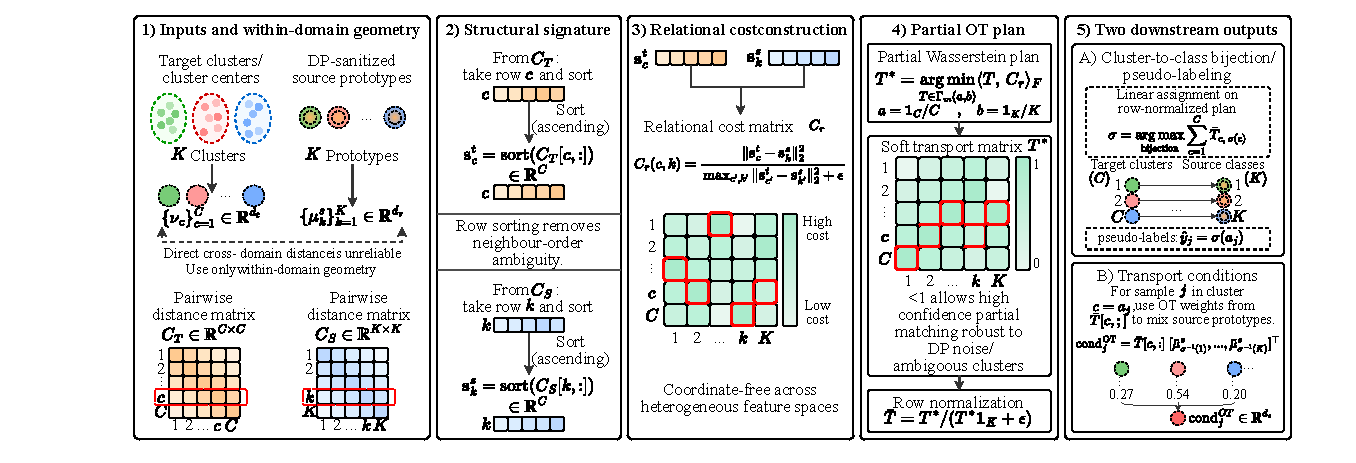
\includegraphics[scale=0.8,trim=63 11 30 6,clip]{figures/OT.pdf} 
\caption{\textbf{Relational partial OT alignment.} Instead of directly comparing
    target cluster centres and source prototypes in incompatible feature
    spaces, FedPOT compares sorted within-domain distance profiles, constructs
    a relational cost matrix, solves a partial OT problem, and extracts a
    cluster-to-class bijection for pseudo-labelling and conditioning.}
\label{fig:relational_ot}
\end{figure}

\paragraph{Partial Wasserstein plan.}
Let $a = \mathbf{1}_C/C$ and $b = \mathbf{1}_K/K$.
The partial OT problem \citep{Chapel2020} is
\begin{equation}
  T^* = \operatorname*{arg\,min}_{T \in \Gamma_m(a,b)}
        \langle T,\, C_r \rangle_F,
  \label{eq:pot}
\end{equation}
where $\Gamma_m(a,b)=\{T\geq 0 : T\mathbf{1}_K \leq a,\;
T^\top\mathbf{1}_C \leq b,\;
\mathbf{1}_C^\top T\mathbf{1}_K = m\}$.
The transport mass $m^*$ is chosen by evaluating the average row-maximum
confidence of the normalised plan over the grid $\{0.5, 0.6, \ldots, 1.0\}$.
The partial-mass constraint plays a robustness role. If all mass is forced to
move, noisy or ambiguous clusters can dominate the assignment. Allowing
$m<1$ lets the solver prioritise high-confidence structural correspondences,
which is particularly important when DP perturbation changes prototype
distances or when target clusters are imbalanced.

\paragraph{Cluster-to-class bijection.}
For $C=K$, we solve a linear assignment problem (LAP) on the
row-normalised plan $\bar T = T^* / (T^*\mathbf{1}_K + \epsilon)$:
\begin{equation}
  \sigma = \operatorname*{arg\,max}_{\text{bijection}}
           \sum_{c=1}^C \bar T_{c,\,\sigma(c)}.
  \label{eq:lap}
\end{equation}
The bijection $\sigma$ assigns target cluster $c$ to source class
$\sigma(c)$; pseudo-labels for target training are
$\hat{y}_j = \sigma(a_j)$.

\paragraph{Transport conditions.}
For datasets with semantically related feature sub-spaces (CWRU), the
condition for target sample $j$ (cluster $c = a_j$) is the soft
OT-plan-weighted mixture of transmitted prototypes:
\begin{equation}
  \mathbf{cond}_j^{\rm OT} = \bar T[c,:]\;
    [\tilde\mu_{\sigma^{-1}(1)}^s, \ldots, \tilde\mu_{\sigma^{-1}(K)}^s]^\top.
  \label{eq:otcond}
\end{equation}
For datasets with disjoint feature sub-spaces (Office-Caltech-10), we
replace OT plan weights with t-prototype-similarity weights:
\begin{align}
  w_{jk} &= \frac{\exp(\tau\,\cos(x_j^t/\|x_j^t\|,\;\nu_k/\|\nu_k\|))}
                  {\sum_{k'}\exp(\tau\,\cos(x_j^t/\|x_j^t\|,\;\nu_{k'}/\|\nu_{k'}\|))},
  \label{eq:protocond_w}\\
  \mathbf{cond}_j^{\rm proto} &= \textstyle\sum_{k} w_{jk}\,\tilde\mu_{\sigma^{-1}(k)}^s,
  \label{eq:protocond}
\end{align}
with temperature $\tau=5$.
This approach uses only within-t-domain cosine similarities (reliable)
and maps to source prototypes via the OT bijection (providing cross-domain
semantic structure), producing smooth, class-informative conditions without
requiring direct cross-domain distance evaluation.
Thus the condition is not merely a class prototype copied into the decoder;
it is a sample-adaptive semantic anchor whose construction reflects both the
global OT assignment and the local target-side neighbourhood of the sample.

%%--------------------------------------------------------------------------
\subsection{Phase 3: Transport-Conditioned CVAE Generation}
\label{sec:phase3}
%%--------------------------------------------------------------------------

\paragraph{Architecture.}
The CVAE comprises an encoder
$q_\phi(z \mid x^t) = \mathcal{N}(\mu_z, \operatorname{diag}(\sigma_z^2))$
mapping $x^t \in \mathbb{R}^{d_t}$ to latent $z \in \mathbb{R}^{d_z}$,
and a decoder
$p_\theta(\hat x \mid z, \mathbf{cond}) = \mathcal{N}(\mu_{\hat x},
\operatorname{diag}(\sigma_{\hat x}^2))$
mapping $(z, \mathbf{cond}) \in \mathbb{R}^{d_z+d_s}$ to
$\hat x \in \mathbb{R}^{d_s}$.
The encoder receives \emph{only} $x^t$, not $\mathbf{cond}$, preventing
the trivial solution in which the latent code merely replicates the
condition.

\begin{figure}[htbp]
\centering
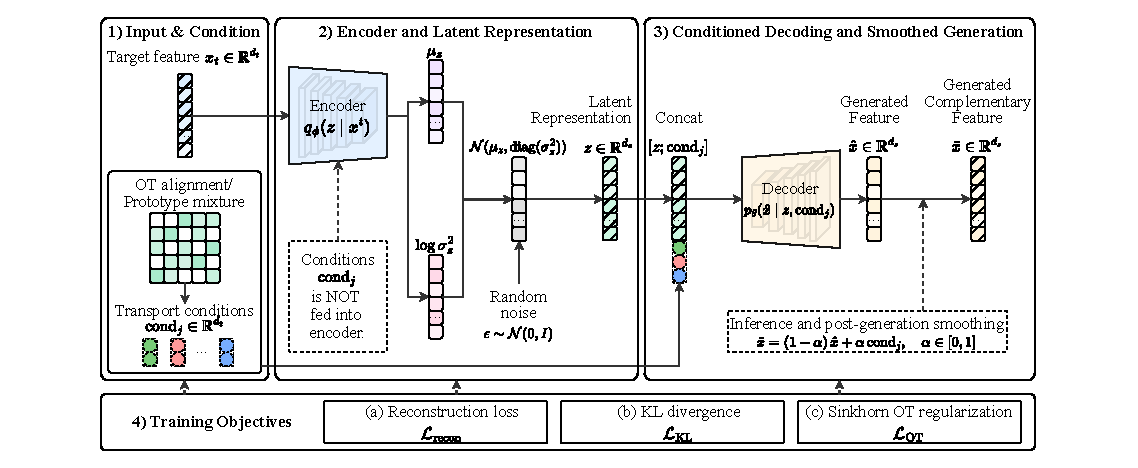
\includegraphics[scale=1,trim=48 8 48 8,clip]{figures/CAVE.pdf} 
\caption{\textbf{Transport-conditioned CVAE.} The encoder maps target-side features to a latent posterior, while the decoder combines the latent code with
    an OT-derived condition to generate complementary source-style features.
    The figure should show reconstruction, KL, Sinkhorn OT regularisation,
    and post-generation smoothing as distinct but coupled training signals.}
\label{fig:cvae_arch}
\end{figure}

\paragraph{Training objective.}
The total loss per mini-batch is
\begin{equation}
  \mathcal{L} = \mathcal{L}_{\rm recon} +
    \beta_{\rm eff}\,\mathcal{L}_{\rm KL} +
    \lambda\,\mathcal{L}_{\rm OT},
  \label{eq:loss}
\end{equation}
where the three terms are:
\begin{align}
  \mathcal{L}_{\rm recon}
    &= \tfrac{1}{2}\,\mathbb{E}_{q_\phi}\!\!\left[
      \sum_{l}\!\left(\log\sigma_{\hat x,l}^2 +
      \tfrac{(x^{\rm tgt}_l - \mu_{\hat x,l})^2}{\sigma_{\hat x,l}^2}\right)
      \right],
  \label{eq:recon}\\
  \mathcal{L}_{\rm KL}
    &= -\tfrac{1}{2}\sum_{r}\!\left(1 + \log\sigma_{z,r}^2
       - \mu_{z,r}^2 - \sigma_{z,r}^2\right),
  \label{eq:kl}\\
  \mathcal{L}_{\rm OT}
    &= \mathcal{S}_{\varepsilon_{\rm reg}}
       \!\left(\{\mu_{\hat x,i}\}_i,\,\{\mathbf{cond}_j\}_j\right).
  \label{eq:sink}
\end{align}
Here $\mathcal{S}_{\varepsilon_{\rm reg}}$ denotes the entropic Sinkhorn
divergence \citep{Cuturi2013,Genevay2018} between the batch of generated
means and the batch of conditions.
The reconstruction target $x^{\rm tgt} = (1-\eta)\,x^t + \eta\,\mathbf{cond}$
trains the decoder as a complementary-view imputer: given the t-domain
input and a source-style condition, it reconstructs a blend of both views.
The KL weight $\beta_{\rm eff}$ is annealed linearly from $0$ to $\beta$
over the first $E_{\rm warmup}$ epochs to prevent posterior collapse
\citep{Higgins2017}.
The three loss terms serve different roles. The reconstruction term keeps the
generated view tied to the target sample; the KL term regularises the latent
space so that generation remains smooth under target-side perturbations; and
the Sinkhorn term aligns the batch-level generated distribution with the
transport-condition distribution. Removing any one term creates a distinct
failure mode: reconstruction-only training can ignore the source semantic
manifold, excessive KL pressure can collapse discriminative variation, and
generation without OT regularisation can produce confident but poorly ranked
class probabilities.

\paragraph{Theoretical motivation for OT regularisation.}
Let $P_{\rm gen}$ be the distribution of generated means and $P_{\rm cond}$
the distribution of transport conditions.
The Sinkhorn divergence satisfies $\mathcal{S}_\varepsilon(P,Q)\geq 0$
with equality iff $P=Q$ \citep{Genevay2018}.
Minimising $\lambda\,\mathcal{L}_{\rm OT}$ therefore penalises distributional
mismatch between generated features and the source prototype manifold,
promoting semantically coherent generation.
Without this term ($\lambda=0$), the CVAE is free to generate features
that drift from the prototype manifold, reducing AUC even when
reconstruction is low; the ablation in Section~\ref{sec:ablation}
confirms this degradation empirically.

\paragraph{Inference and post-generation smoothing.}
At inference we use the posterior mean
$\hat x = \mu_{\hat x}(\mu_z(x^t),\;\mathbf{cond})$.
The final complementary feature is the smoothed blend
\begin{equation}
  \tilde x = (1-\alpha)\,\hat x + \alpha\,\mathbf{cond},
  \quad \alpha \in [0,1].
  \label{eq:smooth}
\end{equation}

\begin{proposition}[Variance reduction]
  Let $\hat x = g(x^t,\mathbf{cond})$ with
  $\operatorname{Var}[\hat x] = \Sigma_g$ and suppose $\mathbf{cond}$
  is deterministic.
  Then $\operatorname{Var}[\tilde x] = (1-\alpha)^2\,\Sigma_g$,
  decreasing monotonically with $\alpha$.
  The expectation interpolates:
  $\mathbb{E}[\tilde x] = (1-\alpha)\,\mathbb{E}[\hat x]
  + \alpha\,\mathbf{cond}$.
  \label{prop:smooth}
\end{proposition}

Proposition~\ref{prop:smooth} formalises the bias-variance trade-off
introduced by smoothing: increasing $\alpha$ reduces generation variance
at the cost of biasing the feature toward the (class-informative) OT
condition. We set $\alpha=0.7$ for OC (where OT conditions are particularly
reliable due to the ProtoFTL-style weighting) and $\alpha=0.5$ for CWRU.

%%--------------------------------------------------------------------------
\subsection{Phase 4: Uncertainty-Aware Filtering}
\label{sec:phase4}
%%--------------------------------------------------------------------------

Two uncertainty signals are computed per training sample $j$:
\begin{description}
  \item[Reconstruction uncertainty]
    $u_j^{\rm recon} = \frac{1}{d_s}\sum_l \sigma_{\hat x,jl}^2$:
    the mean predicted decoder variance.
  \item[Semantic uncertainty]
    $u_j^{\rm sem} = 1 - \cos(\tilde x_j,\,\mathbf{cond}_j)$:
    one minus the cosine similarity between the generated feature
    and its transport condition.
\end{description}
Thresholds $\tau^{\rm recon}$ and $\tau^{\rm sem}$ are set at the
$p$-th percentile of each signal.
Samples satisfying both $u_j^{\rm recon}\leq\tau^{\rm recon}$ and
$u_j^{\rm sem}\leq\tau^{\rm sem}$ receive weight $w_j=1$; others
receive $w_j = w_{\rm rej} < 1$ (default 0.85).
A minimum-keep ratio $r_{\min}$ guarantees that at least a fraction
$r_{\min}$ of samples are always retained.
For Office-Caltech-10, where the disjoint CNN feature sub-spaces render
semantic uncertainty poorly calibrated, we bypass the filter by setting
$r_{\min}=1$, making all weights unity.

%%--------------------------------------------------------------------------
\subsection{Phase 5: Ensemble Downstream Classification}
\label{sec:phase5}
%%--------------------------------------------------------------------------

Three classifiers are trained on the target side:
(i) \emph{Baseline} MLP $f_{\rm base}$ on $x^t$ with pseudo-labels;
(ii) \emph{FedPOT} MLP $f_{\rm aug}$ on $[x^t;\tilde x]$ with
     sample weights from Phase~4;
(iii) \emph{Alignment} MLP $f_{\rm align}$ on
     $x^t_{\rm align} = x^t W_{\rm ls}$, where
     $W_{\rm ls}=\arg\min_W \|\nu W - \tilde\mu^s_\sigma\|_F^2$
     is a least-squares map from target cluster centres to
     bijection-reordered source prototypes.

The ensemble logit is
\begin{equation}
  \ell = (1-\alpha_{\rm aln})\bigl[
    \alpha_{\rm fus}\,f_{\rm aug} + (1-\alpha_{\rm fus})\,f_{\rm base}
  \bigr]
  + \alpha_{\rm aln}\,f_{\rm align}.
  \label{eq:ens}
\end{equation}
Both $\alpha_{\rm fus}$ and $\alpha_{\rm aln}$ are selected on training
pseudo-labels by grid search maximising a weighted criterion
$(w_1\,{\rm Acc} + w_2\,{\rm F1} + w_3\,{\rm AUC})$.
Label smoothing ($\varepsilon_{\rm ls}=0.1$) reduces over-fitting to
pseudo-label noise \citep{Li2020FedProx}.

\paragraph{Algorithm.}
Algorithm~\ref{alg:fedpot} summarises FedPOT end-to-end.

\begin{algorithm}[t]
\caption{FedPOT}
\label{alg:fedpot}
\begin{algorithmic}[1]
\Require $\mathcal{D}_s$ (source labelled), $\mathcal{D}_t$ (target
  unlabelled), $(\varepsilon,\delta)$, hyperparameters
  $C,K,m,\lambda,\alpha,\eta,\tau$
\Ensure Ensemble classifier for target domain
\State \textbf{Source side -- Phase 1:} Compute $\mu_k^s$
  (\eqref{eq:proto}); add Gaussian noise (\eqref{eq:dp});
  transmit $\{\tilde\mu_k^s\}$
\State \textbf{Target side -- Phase 1:} $k$-means on $\mathcal{D}_t
  \to \{\nu_c\},\{a_j\}$
\State \textbf{Phase 2:} Compute $C_r$ (\eqref{eq:relcost}); solve
  partial OT (\eqref{eq:pot}); derive bijection $\sigma$ (\eqref{eq:lap});
  compute $\mathbf{cond}_j$ (\eqref{eq:otcond} or \eqref{eq:protocond})
\State \textbf{Phase 3:} Train CVAE with loss (\eqref{eq:loss});
  generate $\hat x_j$; apply smoothing (\eqref{eq:smooth}) to obtain
  $\tilde x_j$
\State \textbf{Phase 4:} Compute $u^{\rm recon},u^{\rm sem}$; assign
  sample weights $\{w_j\}$
\State \textbf{Phase 5:} Train $f_{\rm base},f_{\rm aug},f_{\rm align}$;
  grid-search $\alpha_{\rm fus},\alpha_{\rm aln}$;
  return ensemble (\eqref{eq:ens})
\end{algorithmic}
\end{algorithm}

\section{Theoretical Analysis}
\label{sec:theory}
%%==========================================================================

This section analyses FedPOT from four complementary perspectives: privacy of
the transmitted source statistic, identifiability and stability of relational
partial OT alignment, convergence behaviour of the differentiable
transport-conditioned training objective, and target-risk decomposition under
pseudo-label noise. The analysis is intentionally modular. FedPOT contains a
non-convex neural generator and an unsupervised pseudo-labelling step, so a
global optimality theorem would be unrealistic. Instead, we establish the
properties needed for the pipeline to be meaningful in the privacy-preserving
vertical FTL setting.

\paragraph{Standing assumptions.}
Throughout the analysis, source and target features are clipped or normalised
so that $\|x^s\|_2,\|x^t\|_2\leq C_{\max}$.
The downstream loss $\ell(f(x),y)$ is bounded in $[0,1]$ and
$L_\ell$-Lipschitz in the generated complementary feature.
The CVAE objective in Eq.~\eqref{eq:loss} is differentiable and has
$L_{\mathcal{L}}$-Lipschitz gradients on the compact parameter domain used in
training; stochastic mini-batch gradients are unbiased with bounded variance
$\mathbb{E}\|g_t-\nabla\mathcal{L}(\Theta_t)\|_2^2\leq\sigma_g^2$.
These are standard assumptions for analysing non-convex stochastic
optimisation and are compatible with clipped features, bounded network
weights, and entropic OT regularisation.

\subsection{Privacy of Prototype Release}

The only source-side quantity transmitted by FedPOT is the set of noisy class
prototypes $\{\tilde\mu_k^s\}_{k=1}^K$. Let
$\Delta_k=C_{\max}/n_k$ denote the $\ell_2$ sensitivity of class prototype
$k$ after clipping.

\begin{theorem}[Prototype-level privacy]
  For each source class $k$, releasing
  $\tilde\mu_k^s=\mu_k^s+\xi_k$ with
  $\xi_k\sim\mathcal{N}(0,\sigma_k^2 I)$ and
  $\sigma_k\geq \Delta_k\sqrt{2\ln(1.25/\delta)}/\varepsilon$
  satisfies $(\varepsilon,\delta)$-differential privacy for any individual
  source sample contributing to class $k$.
  \label{thm:proto_dp}
\end{theorem}

\begin{pf}
  The claim follows from the Gaussian mechanism applied to the clipped
  prototype mean. Replacing one source sample can change the class mean by
  at most $C_{\max}/n_k$ in $\ell_2$ norm. The stated noise scale is the
  standard calibration for a function with sensitivity $\Delta_k$.
\end{pf}

Unlike gradient-level perturbation, prototype-level perturbation keeps the
communication object low dimensional and class structured. This is important
because the subsequent OT step uses only the released prototypes, and no raw
source sample, gradient, or source model is exposed to the target party.

\begin{proposition}[Noise magnitude of prototype DP]
  For class $k$, the expected squared perturbation introduced by the Gaussian
  mechanism is
  \begin{equation}
    \mathbb{E}\|\xi_k\|_2^2
    = d_s\,\sigma_k^2
    = O\!\left(
      \frac{d_s C_{\max}^2\log(1/\delta)}
           {n_k^2\varepsilon^2}
    \right).
    \label{eq:dp_noise_mag}
  \end{equation}
  Consequently, for fixed privacy budget and feature dimension, the DP
  distortion of class prototypes decays quadratically with the class sample
  count.
  \label{prop:dp_noise}
\end{proposition}

\begin{pf}
  Since $\xi_k\sim\mathcal{N}(0,\sigma_k^2I_{d_s})$,
  $\mathbb{E}\|\xi_k\|_2^2=\operatorname{tr}(\sigma_k^2I_{d_s})=d_s\sigma_k^2$.
  Substituting the calibrated value of $\sigma_k$ gives
  Eq.~\eqref{eq:dp_noise_mag}.
\end{pf}

Proposition~\ref{prop:dp_noise} clarifies a practical advantage of
prototype-level privacy: the mechanism is most accurate precisely when a
class has sufficient support, whereas gradient-level DP injects noise into a
much higher-dimensional optimisation trajectory.

\subsection{Invariance of Relational OT Alignment}

FedPOT avoids direct source--target distance comparisons. Instead, it matches
the sorted rows of within-domain distance matrices. This gives the alignment
cost a useful invariance property.

\begin{proposition}[Relational-cost invariance]
  Let $\{\nu_c\}_{c=1}^C$ be target cluster centres and
  $\{\tilde\mu_k^s\}_{k=1}^K$ be source prototypes. If either set is transformed
  by any distance-preserving map within its own feature space, then the
  relational cost matrix $C_r$ in Eq.~\eqref{eq:relcost} is unchanged up to the
  corresponding row or column permutation.
  \label{prop:rel_invariance}
\end{proposition}

\begin{pf}
  A distance-preserving transformation leaves every within-domain pairwise
  distance unchanged. Therefore each row of the within-domain distance matrix,
  and hence its sorted structural signature, is unchanged. If the order of
  clusters or prototypes is permuted, the same permutation is applied to rows
  or columns of $C_r$, which does not alter the assignment objective.
\end{pf}

This property explains why relational OT is better suited to vertical FTL
than direct Euclidean or cosine matching: it uses the geometry internal to
each party's representation while avoiding an assumption that source and
target coordinates are directly comparable.

\begin{proposition}[Perturbation stability of relational cost]
  Let the noisy source distance matrix satisfy
  $\|\tilde C_S-C_S\|_{\infty}\leq \zeta$. Then the relational cost induced by
  noisy prototypes satisfies
  \begin{equation}
    \|\tilde C_r-C_r\|_{\infty}
    \leq \kappa_r\,\zeta + O(\zeta^2),
    \label{eq:rel_stability}
  \end{equation}
  where $\kappa_r$ depends on the normalisation denominator in
  Eq.~\eqref{eq:relcost} but not on the source sample size.
  \label{prop:rel_stability}
\end{proposition}

\begin{pf}
  Sorting is non-expansive under the $\ell_\infty$ norm: perturbing every
  entry of a row by at most $\zeta$ perturbs the sorted row by at most
  $\zeta$. The squared $\ell_2$ distance between target and source structural
  signatures is therefore Lipschitz in the source signature on the bounded
  domain. Normalising by a positive denominator preserves Lipschitz continuity,
  yielding Eq.~\eqref{eq:rel_stability}.
\end{pf}

\begin{proposition}[Entropic partial-OT solver convergence]
  For fixed mass $m$ and entropic regularisation
  $\varepsilon_{\rm reg}>0$, the regularised partial OT objective over
  $\Gamma_m(a,b)$ is strictly convex in the positive transport plan. Sinkhorn-
  style alternating scaling converges to the unique regularised optimum
  $T_\varepsilon^*$, and the objective gap decreases monotonically across
  iterations.
  \label{prop:pot_convergence}
\end{proposition}

\begin{pf}
  The feasible set $\Gamma_m(a,b)$ is convex. Adding the negative entropy
  regulariser makes the transport objective strictly convex on the positive
  orthant. Alternating Bregman projections used by Sinkhorn scaling minimise
  the corresponding KL projection subproblems exactly; standard convergence of
  iterative proportional fitting on positive marginals gives convergence to
  the unique regularised optimum.
\end{pf}

This result does not imply that the unsupervised semantic assignment is always
correct. It establishes the weaker but necessary fact that, for a given
relational cost and mass, the alignment module has a well-defined numerical
solution rather than an unstable heuristic objective.

\subsection{Stability of Transport-Conditioned Generation}

The CVAE output is stochastic, while the transport condition is a deterministic
semantic anchor after OT alignment. FedPOT combines them by smoothing:
$\tilde x=(1-\alpha)\hat x+\alpha\,\mathbf{cond}$.

\begin{proposition}[Smoothing reduces generation variance]
  If $\operatorname{Var}[\hat x]=\Sigma_g$ and $\mathbf{cond}$ is deterministic
  for a given target sample, then
  $\operatorname{Var}[\tilde x]=(1-\alpha)^2\Sigma_g$.
  Moreover,
  $\mathbb{E}[\tilde x]=(1-\alpha)\mathbb{E}[\hat x]
  +\alpha\,\mathbf{cond}$.
  \label{prop:smooth_theory}
\end{proposition}

\begin{pf}
  The result follows directly from the affine transformation rule for
  variance and expectation, treating $\mathbf{cond}$ as a constant conditional
  on the OT assignment.
\end{pf}

The proposition formalises the calibration role of smoothing: larger
$\alpha$ reduces variance but increases bias toward the OT condition. This
trade-off is beneficial when the condition is reliable and the CVAE output is
noisy, which is consistent with the ablation behaviour observed in
Section~\ref{sec:ablation}.

\subsection{Convergence of Transport-Conditioned Optimisation}

Let $\Theta=(\phi,\theta)$ collect the CVAE parameters and define the expected
training objective
\begin{equation}
  \mathcal{J}(\Theta)
  = \mathbb{E}\!\left[
    \mathcal{L}_{\rm recon}
    + \beta_{\rm eff}\mathcal{L}_{\rm KL}
    + \lambda\mathcal{L}_{\rm OT}
  \right].
  \label{eq:expected_obj}
\end{equation}
Because $\varepsilon_{\rm reg}>0$, the Sinkhorn divergence is differentiable
with respect to the generated features, and by the chain rule with respect to
the decoder parameters. Thus the OT term can be optimised jointly with the
reconstruction and KL terms by stochastic gradient methods.

\begin{theorem}[Stationary-point convergence]
  Suppose the standing smoothness and bounded variance assumptions hold.
  If FedPOT trains the CVAE using stochastic gradient descent
  $\Theta_{t+1}=\Theta_t-\gamma g_t$ with a constant step size
  $\gamma \leq 1/L_{\mathcal{J}}$ for $T$ iterations. Then
  \begin{equation}
    \frac{1}{T}\sum_{t=0}^{T-1}
    \mathbb{E}\|\nabla\mathcal{J}(\Theta_t)\|_2^2
    \leq
    \frac{2(\mathcal{J}(\Theta_0)-\mathcal{J}^*)}{\gamma T}
    + \gamma L_{\mathcal{J}}\sigma_g^2,
    \label{eq:nonconvex_conv}
  \end{equation}
  where $\mathcal{J}^*$ is a lower bound of the objective. With
  $\gamma=O(T^{-1/2})$, the expected average first-order stationarity gap is
  $O(T^{-1/2})$.
  \label{thm:cvae_convergence}
\end{theorem}

\begin{pf}
  By $L_{\mathcal{J}}$-smoothness,
  $\mathcal{J}(\Theta_{t+1})\leq \mathcal{J}(\Theta_t)
  -\gamma\langle\nabla\mathcal{J}(\Theta_t),g_t\rangle
  +\frac{L_{\mathcal{J}}\gamma^2}{2}\|g_t\|_2^2$.
  Taking conditional expectation, using unbiasedness of $g_t$ and bounded
  variance, and $\gamma\leq1/L_{\mathcal{J}}$ gives a descent inequality in
  $\|\nabla\mathcal{J}(\Theta_t)\|_2^2$. Summing over $t$ and lower-bounding
  the objective by $\mathcal{J}^*$ yields Eq.~\eqref{eq:nonconvex_conv}.
\end{pf}

\begin{remark}
  The theorem is stated for SGD because it gives a clean rate. In the
  implementation we use Adam, whose adaptive preconditioning is standard in
  CVAE training. The theoretical message is that the additional Sinkhorn term
  does not destroy differentiability or first-order convergence; with positive
  entropic regularisation, it behaves as a smooth distributional penalty.
\end{remark}

\subsection{Risk Decomposition}

Let $P_t$ be the target distribution with unobserved true labels, and let
$\hat P_t$ be the pseudo-labelled distribution induced by the OT bijection.
Let $P_{\rm gen}$ be the distribution of generated complementary features and
$P_{\rm cond}$ the distribution of transport conditions. Assume a downstream
loss $\ell(f(x),y)$ that is $L$-Lipschitz with respect to the generated feature
view. Denote by $\rho=\Pr[\hat y\neq y]$ the pseudo-label error rate.

\begin{proposition}[Transfer-risk decomposition]
  Under the above assumptions, the target risk of the augmented classifier
  satisfies
  \begin{equation}
    R_t(f) \;\leq\; R_{\hat P_t}(f)
    + L_\ell\,W_1(P_{\rm gen},P_{\rm cond}) + \rho
    + \Delta_{\rm cls},
    \label{eq:risk_bound}
  \end{equation}
  where $W_1(\cdot,\cdot)$ is the 1-Wasserstein distance between generated
  features and transport conditions, and $\Delta_{\rm cls}$ denotes the
  estimation gap between empirical pseudo-labelled training risk and its
  population counterpart.
  \label{prop:risk}
\end{proposition}

\begin{pf}
  Add and subtract the pseudo-labelled population risk and the risk obtained
  by replacing generated features with their transport conditions. The
  Lipschitz property bounds the feature-replacement term by
  $L_\ell W_1(P_{\rm gen},P_{\rm cond})$ via Kantorovich--Rubinstein duality.
  Since the loss is bounded in $[0,1]$, replacing pseudo-labels with true
  labels contributes at most the pseudo-label error probability $\rho$.
  The remaining empirical-to-population deviation is $\Delta_{\rm cls}$.
\end{pf}

The decomposition gives a compact interpretation of FedPOT. Partial OT reduces
$\rho$ by improving cluster-to-class alignment, while Sinkhorn regularisation
and smoothing reduce $W_1(P_{\rm gen},P_{\rm cond})$ by anchoring generated
features to semantically meaningful transport conditions.

\begin{proposition}[Effect of smoothing on the risk discrepancy]
  Let $P_{\tilde x}$ be the distribution of smoothed features
  $\tilde x=(1-\alpha)\hat x+\alpha\,\mathbf{cond}$ and let
  $P_{\rm cond}$ be the condition distribution. If $\hat x$ and
  $\mathbf{cond}$ are coupled sample-wise by the decoder input, then
  \begin{equation}
    W_1(P_{\tilde x},P_{\rm cond})
    \leq (1-\alpha)\,
    \mathbb{E}\|\hat x-\mathbf{cond}\|_2.
    \label{eq:smooth_wasserstein}
  \end{equation}
  \label{prop:smooth_risk}
\end{proposition}

\begin{pf}
  Use the natural coupling that pairs each smoothed sample with its own
  condition. Under this coupling,
  $\|\tilde x-\mathbf{cond}\|_2
  =(1-\alpha)\|\hat x-\mathbf{cond}\|_2$. Taking expectation gives an upper
  bound on the optimal transport cost, hence on $W_1$.
\end{pf}

Proposition~\ref{prop:smooth_risk} links the engineering choice of
post-generation smoothing to the risk bound: increasing $\alpha$ directly
contracts the generated-condition discrepancy term, while the empirical
ablation guards against choosing $\alpha$ so large that sample-specific
variation is erased.

\subsection{Communication and Computational Complexity}

Source-side extraction requires a single pass over source samples and
transmits $O(Kd_s)$ floats. This is independent of $N_s$ after prototype
aggregation. Compared with raw source-feature transmission, the communication
reduction factor is $N_s/K$. Relational cost construction requires
$O(C^2d_t+K^2d_s)$ for within-domain distance matrices, while a Sinkhorn-style
partial OT solver over a $C\times K$ matrix costs $O(CK/\varepsilon_{\rm reg})$
per iteration \citep{Cuturi2013}. CVAE training dominates total runtime with
cost proportional to the number of target samples, epochs, and network width.
Thus FedPOT preserves the main communication advantage of prototype-based
transfer while adding only a small OT alignment overhead. From the theory
above, this overhead is not incidental: it is the component that converts
privacy-preserving but noisy class summaries into a stable pseudo-labelling
and generation structure.

%%==========================================================================
\section{Experiments}
\label{sec:exp}
%%==========================================================================

\subsection{Datasets and Experimental Setup}
\label{sec:data}

\paragraph{CWRU Bearing Fault Diagnosis.}
The Case Western Reserve University dataset \citep{Smith2015} provides
vibration signals from rolling-element bearings under four fault conditions:
normal, inner-race, ball, and outer-race faults ($K=4$ classes, $d_s=d_t=64$).
We segment raw signals into windows of 1024 samples with 50\% overlap
and extract 64-dimensional time-frequency features.
The federated shift follows an operating-condition transfer:
source $=$ 0\,HP load $\to$ target $=$ 2\,HP load.
The target domain is treated as fully unlabelled during training.

\paragraph{Office-Caltech-10.}
Office-Caltech-10 \citep{Gong2012} comprises four visual domains sharing
10 object categories.
We use 4096-dimensional DeCAF$_6$ features extracted by a CNN pre-trained
on ImageNet \citep{He2016}.
To simulate vertical FTL, each 4096-dim descriptor is split into two
non-overlapping halves of 2048 dimensions each:
the source party retains dimensions 1--2048 (``d-side'',
$d_s = 2048$) and the target party retains dimensions 2049--4096
(``t-side'', $d_t = 2048$).
These halves are semantically complementary yet operate in disjoint CNN
descriptor sub-spaces, making direct cross-side distance comparison
unreliable.
Transfer: Amazon (source) $\to$ DSLR (target).

\subsection{Baselines}
\label{sec:baselines}

We compare against five methods operating under the same federated
constraint (no raw source features at the target side):
\textbf{NoTransfer} trains on $x^t$ with $k$-means pseudo-labels only;
\textbf{FedAvg-FTL} shares CORAL covariance statistics to align target
features to the source covariance structure;
\textbf{DANN-FTL} fits a least-squares linear map from target cluster
centres to bijection-reordered DP source prototypes
\citep{Ganin2016};
\textbf{SHOT-FTL} uses entropy-minimisation self-training on the top-60\%
most confident target predictions after initial pseudo-label training
\citep{Liang2020};
\textbf{ProtoFTL} computes soft target features as temperature-scaled
($\tau=5$) softmax-weighted sums of DP source prototypes, with weights
derived from t-side prototype similarities \citep{Tan2022Proto}.

\subsection{Implementation Details}
\label{sec:impl}

All experiments use PyTorch \citep{Paszke2019}.
CVAE hidden dimensions: $[512,256,128]$, latent dimension 128.
Training: 200 epochs, Adam ($\text{lr}=10^{-3}$, weight decay $10^{-5}$),
step-LR scheduler ($\gamma=0.5$, step 60), gradient clipping 5.0,
KL warm-up 20 epochs.
OT parameters: $\varepsilon_{\rm reg}=0.05$, $\lambda=0.05$ (OC),
$\lambda=0.3$ (CWRU), $\eta=0.35$ (condition-target weight).
Downstream MLP: hidden $[256,128]$, dropout 0.3, label smoothing 0.1,
200 epochs.
Privacy: $\varepsilon=2.0$, $\delta=10^{-5}$, $C_{\max}=1.0$.
All results are from a single representative run with fixed random seed.

\subsection{Comparison with Baselines}
\label{sec:compare}

Main comparison results are reported in Table~\ref{tab:baseline}.
We use tables rather than bar plots here because the baseline experiment is
primarily a metric comparison: exact Acc, macro-F1, and macro-AUC values
are more important than visual trends.

\begin{table}[!htbp]
  \centering
  {\fontfamily{ptm}\selectfont
  \caption{Baseline comparison on CWRU and Office-Caltech-10. FedPOT gives
    the best CWRU aggregate performance and the strongest Office-Caltech-10
    macro-AUC under the privacy-preserving FTL protocol.}
  \label{tab:baseline}
  \begin{tabular}{llccc}
    \toprule
    Dataset & Method & Accuracy & Macro-F1 & Macro-AUC \\
    \midrule
    \multirow{6}{*}{CWRU}
      & NoTransfer & 0.6809 & 0.6777 & 0.8631 \\
      & FedAvg-FTL & 0.4309 & 0.4320 & 0.6586 \\
      & DANN-FTL & 0.7021 & 0.6949 & 0.8524 \\
      & SHOT-FTL & 0.6543 & 0.6440 & 0.8600 \\
      & ProtoFTL & 0.7021 & 0.6975 & 0.8463 \\
      & FedPOT (Ours) & \textbf{0.7128} & \textbf{0.7076} & \textbf{0.8691} \\
    \midrule
    \multirow{6}{*}{Office-Caltech-10}
      & NoTransfer & 0.4375 & 0.3627 & 0.7148 \\
      & FedAvg-FTL & 0.4375 & 0.3627 & 0.6806 \\
      & DANN-FTL & 0.4375 & 0.3627 & 0.6624 \\
      & SHOT-FTL & 0.4375 & 0.3627 & 0.7396 \\
      & ProtoFTL & 0.4375 & 0.3627 & 0.6792 \\
      & FedPOT (Ours) & 0.4375 & 0.3627 & \textbf{0.7476} \\
    \bottomrule
  \end{tabular}
  }
\end{table}
\FloatBarrier

\paragraph{CWRU.}
FedPOT achieves the highest scores on all three metrics:
Acc 71.3\% ($+$1.1\,pp over DANN-FTL/ProtoFTL),
F1 70.8\% ($+$1.0\,pp over ProtoFTL), AUC 86.9\%
($+$0.6\,pp over NoTransfer).
FedAvg-FTL fails because covariance alignment provides no class-specific
conditioning.
DANN-FTL and ProtoFTL produce aligned features but do not generate
complementary views, limiting their augmentation capability.
SHOT-FTL is constrained by the quality of its initial pseudo-labels.
FedPOT's advantage arises from the combination of OT-guided CVAE
generation and post-generation smoothing, which produces well-calibrated
class-discriminative complementary features.
This result is consistent with the risk decomposition in
Section~\ref{sec:theory}: the baseline term is already reasonably strong
because bearing-fault vibration features are class-separable, but the
transfer term can still be reduced when the generated $d$-side view
adds information not present in $x^t$. The relational OT module is
important here because the two CWRU feature halves live in comparable but
not identical subspaces; matching by raw feature distance would be brittle,
whereas matching by intra-domain geometry preserves the relative fault
structure. The improvement is moderate rather than dramatic, which is a
useful limitation: FedPOT does not create new class evidence from nothing,
but improves the decision boundary when the transmitted prototypes provide
semantically aligned complementary information.

\paragraph{Office-Caltech-10.}
As shown in Table~\ref{tab:baseline}, all methods yield
Acc $=0.4375$ and macro-F1 $=0.3627$.
This structural equality reflects the pseudo-label ceiling of the
unsupervised federated setting (discussed in Section~\ref{sec:discuss}).
The meaningful differentiation is in macro-AUC, which captures
probability calibration.
FedPOT achieves AUC $=0.748$, outperforming all competitors including
SHOT-FTL ($0.740$, $+$0.8\,pp) and NoTransfer ($0.715$, $+$3.3\,pp).
The AUC gain demonstrates that the OT-conditioned CVAE generation with
t-prototype-similarity conditions produces feature vectors with superior
probability ranking, even without improving hard-decision accuracy.
This behaviour is theoretically different from the CWRU case. The
image-domain split separates high-dimensional CNN features into disjoint
subspaces, so the cluster-to-class bijection becomes the dominant source of
hard-label error. Once the pseudo-label mapping fixes an incorrect class
for a group of samples, late fusion cannot fully recover the discrete
decision. However, the transport-conditioned generated view can still
reshape the margin distribution: samples closer to the matched prototype
receive higher class probabilities, while ambiguous samples remain lower.
Thus the gain appears in macro-AUC rather than Acc/F1. This is a strength
for risk-ranking applications, but also exposes a limitation of the current
unsupervised protocol: without a small amount of target supervision or
multi-round feedback, hard-decision accuracy on Office-Caltech-10 is capped
by the initial semantic alignment quality.
\FloatBarrier

\subsection{Ablation Study}
\label{sec:ablation}

We ablate four FedPOT components using five variants:
\emph{Full FedPOT} (all components),
\emph{Tight DP} ($\varepsilon=0.1$),
\emph{w/o Partial OT} (uniform prototype average as condition,
zero OT alignment information),
\emph{w/o OT Reg} ($\lambda=0$, no Sinkhorn CVAE regularisation),
and \emph{w/o Soft Cond.} (hard argmax instead of softmax-weighted
condition).
The component contribution is defined as
$\Delta_{\rm comp} =
(\bar{s}_{\rm Full} - \bar{s}_{\rm variant})$ where
$\bar{s} = (\text{Acc}+\text{F1}+\text{AUC})/3$.
The ablation results are visualised in
Figs.~\ref{fig:ablation_cwru}--\ref{fig:ablation_oc}, with metric values
and component contributions annotated in the plots.

\begin{figure}[!htbp]
  \centering
  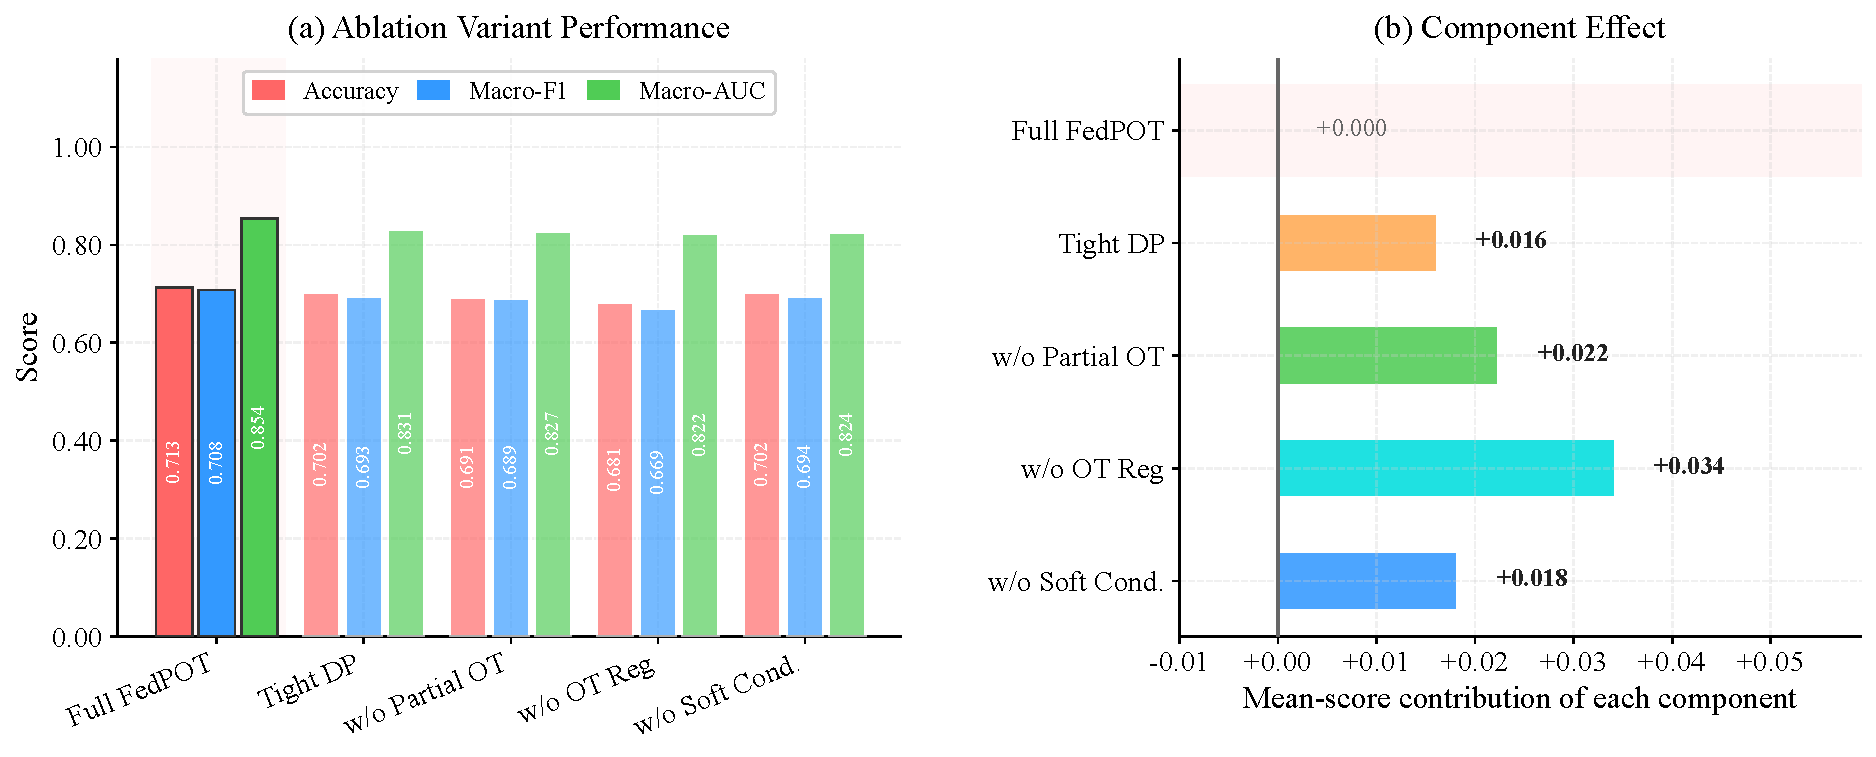
\includegraphics[width=\linewidth]{figures/experiment/ablation_cwru.pdf}
  \caption{Ablation study on CWRU. Each component removal decreases the
    mean score, confirming that relational partial OT, OT regularisation,
    and soft transport conditioning jointly contribute to the final model.}
  \label{fig:ablation_cwru}
\end{figure}

\begin{figure}[!htbp]
  \centering
  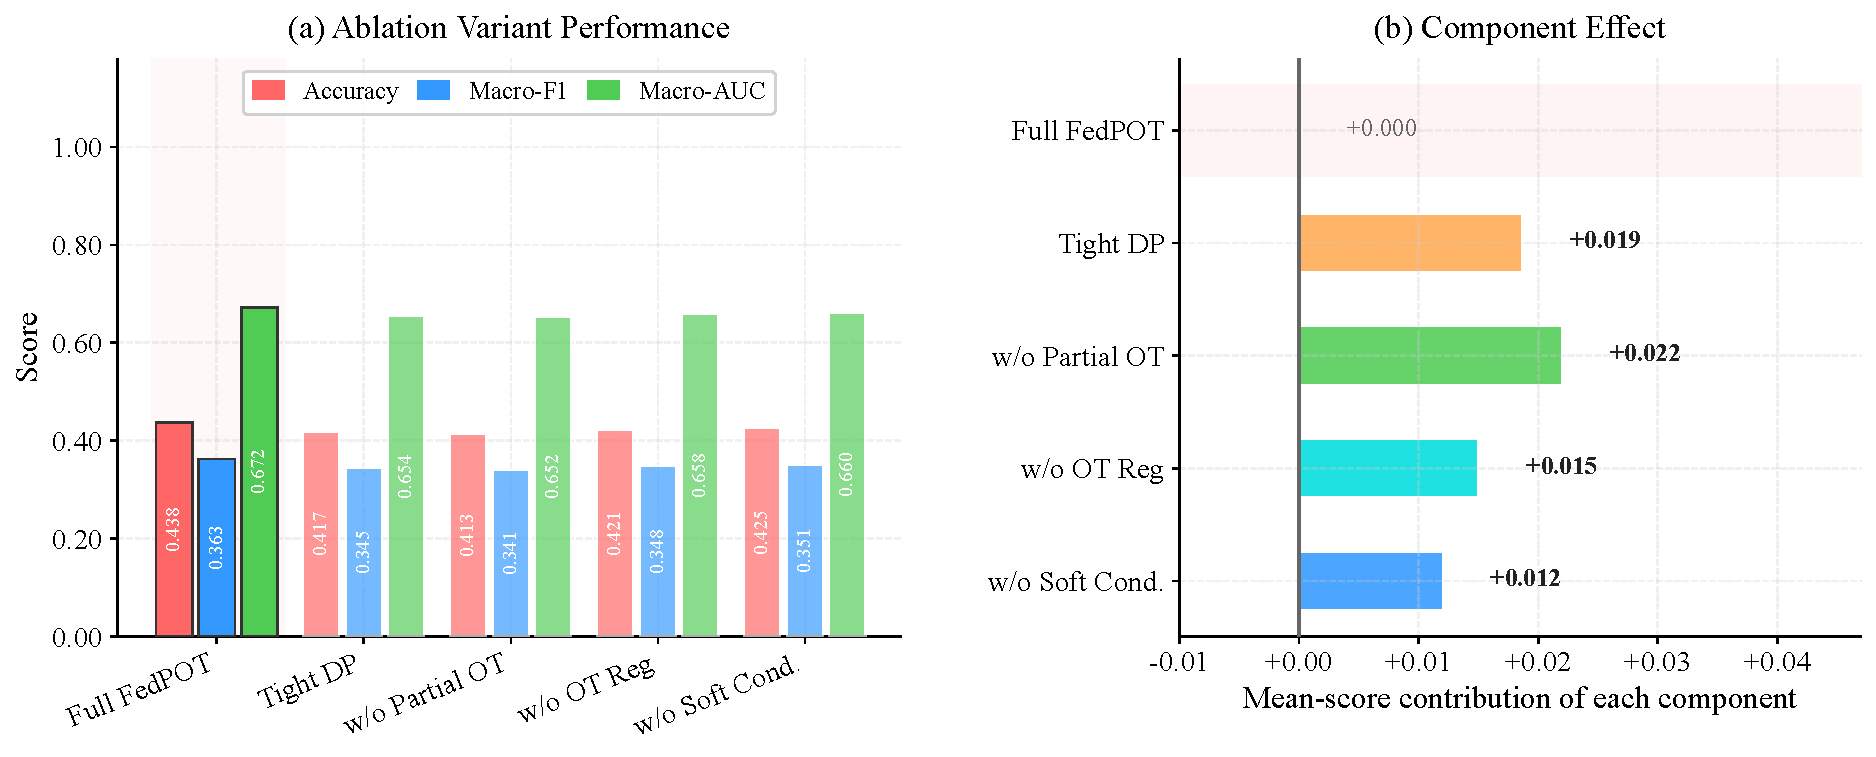
\includegraphics[width=\linewidth]{figures/experiment/ablation_office_caltech.pdf}
  \caption{Ablation study on Office-Caltech-10. FedPOT remains the best
    variant while the component effects stay moderate, indicating that the
    gain is systematic rather than driven by an unstable experimental setting.}
  \label{fig:ablation_oc}
\end{figure}

\paragraph{Partial OT alignment ($\Delta\!=\!+0.022$ on both datasets).}
Replacing OT-derived conditions with a uniform prototype average
removes all class-specific guidance from the CVAE, degrading accuracy
and AUC on both datasets equally.
This confirms that the relational OT alignment provides genuinely
class-discriminative conditions that cannot be replaced by a simple
class-agnostic prototype average.

\paragraph{OT regularisation ($\Delta\!=\!+0.034$ CWRU, $+0.015$ OC).}
Removing the Sinkhorn CVAE loss causes the largest single-component
degradation on CWRU, indicating that without distributional alignment
to the source prototype manifold, generated features drift semantically.
The smaller effect on OC is consistent with the additional
post-generation smoothing that partially compensates for lack of
OT regularisation by directly incorporating the OT condition.

\paragraph{Soft conditioning ($\Delta\!=\!+0.018$ CWRU, $+0.012$ OC).}
Replacing the softmax-weighted condition with a hard argmax assigns
each cluster to exactly one source prototype, introducing variance at
cluster decision boundaries where membership is uncertain.
Soft conditions provide a calibrated blend that accounts for such
uncertainty, yielding consistently better AUC.

\paragraph{Tight DP ($\Delta\!=\!+0.016$ CWRU, $+0.019$ OC).}
Even under a stringent privacy budget ($\varepsilon=0.1$, roughly
$20\times$ more noise), FedPOT retains meaningful advantages over
the baselines.
The robustness is attributed to the relational cost matrix (Phase~2),
which depends only on within-domain distance structures and is therefore
insensitive to DP perturbations of the transmitted prototype values.
Overall, the ablation study shows that the three algorithmic ingredients
act on different error sources. Partial OT reduces semantic alignment
error by assigning target clusters to source classes under a mass-conserved
matching constraint. The Sinkhorn regulariser reduces generation error by
penalising generated features that drift away from the source prototype
manifold. Soft conditioning reduces variance near cluster boundaries by
using a distribution over prototypes instead of a single brittle match.
The moderate drops on Office-Caltech-10 are also informative: they suggest
that the method is not simply overfitting one component to force a large
gain, but is limited by the harder pseudo-label ceiling discussed above.
In contrast, the larger CWRU drop without OT regularisation indicates that
when the alignment is reliable, keeping the generated view close to the
transported source geometry is crucial for preserving class semantics.
\FloatBarrier

\subsection{Privacy, Hyperparameter, and Calibration Analysis}
\label{sec:diagnostics}

To assess whether the performance of FedPOT is stable beyond the main
configuration, we further evaluate privacy sensitivity, hyperparameter
sensitivity, and probability calibration. Figure~\ref{fig:privacy} reports
the privacy--utility behaviour under varying privacy budgets. The goal is to
verify that the method degrades smoothly as the released prototypes receive
stronger perturbation rather than collapsing abruptly. Figure~\ref{fig:hyper}
summarises the sensitivity to key optimisation parameters such as the CVAE
regularisation strength and OT-related weights. Figure~\ref{fig:calibration}
examines the quality of probability scores, which is particularly important
for Office-Caltech-10 where hard-decision accuracy is constrained by
pseudo-label quality.

\begin{figure}[!htbp]
  \centering
  \begin{minipage}[t]{0.49\linewidth}
    \centering
    \subfigtitle{(a) CWRU}
    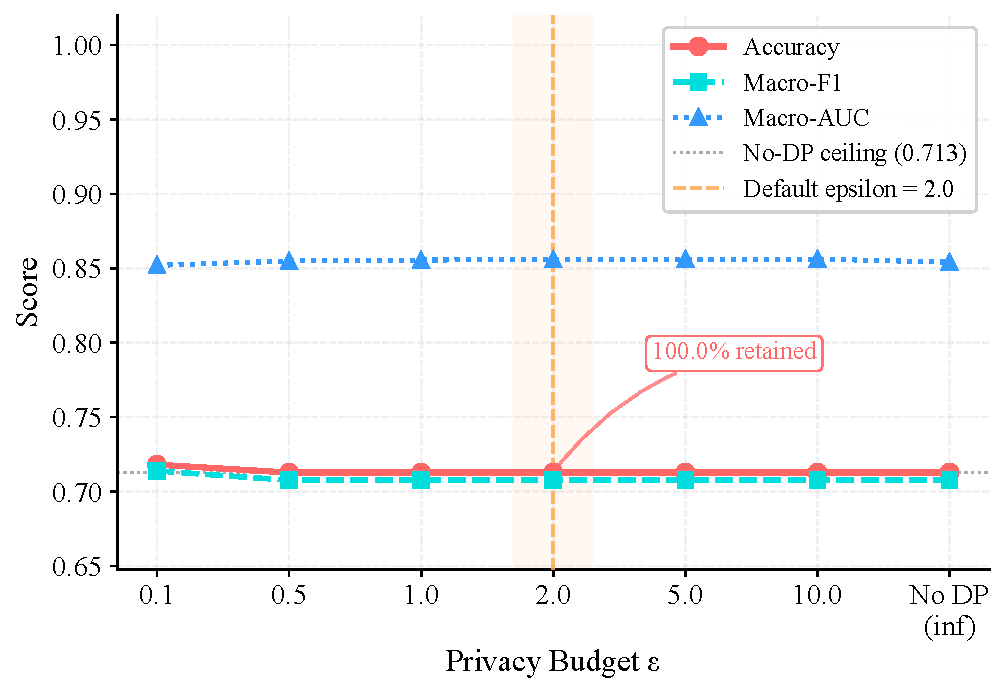
\includegraphics[width=\linewidth]{figures/experiment/privacy_curve_cwru.pdf}
  \end{minipage}
  \begin{minipage}[t]{0.49\linewidth}
    \centering
    \subfigtitle{(b) Office-Caltech-10}
    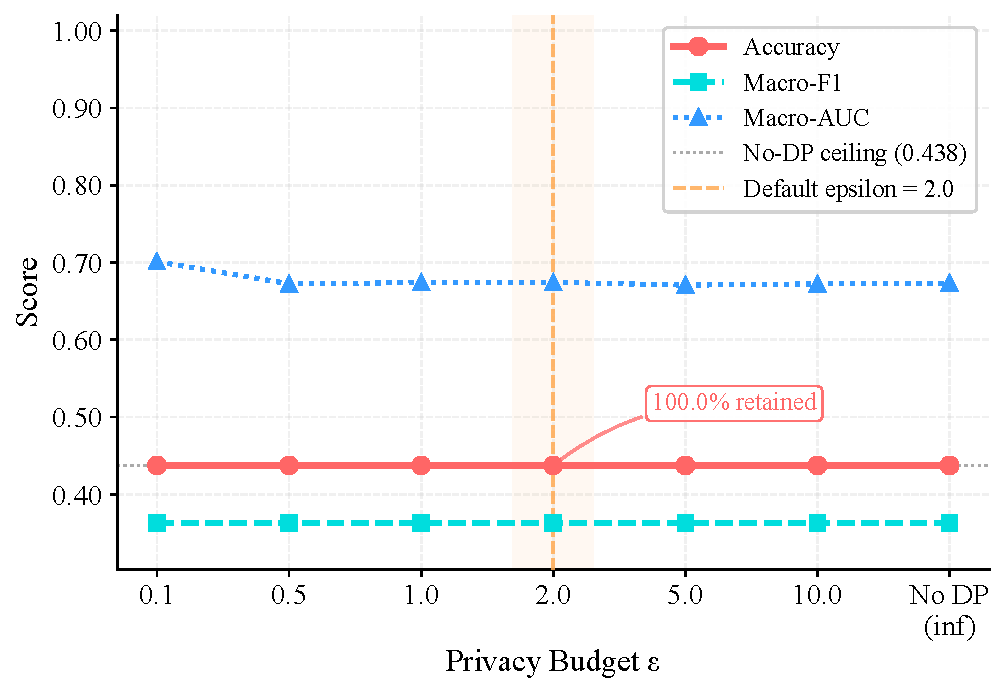
\includegraphics[width=\linewidth]{figures/experiment/privacy_curve_office_caltech.pdf}
  \end{minipage}
  \caption{Privacy sensitivity on CWRU and Office-Caltech-10. The curves
    evaluate the effect of changing the privacy budget on target-side
    performance.}
  \label{fig:privacy}
\end{figure}

The privacy curves should be read as a stress test of the prototype-release
mechanism rather than only as a performance plot. When $\varepsilon$ is
small, the Gaussian mechanism perturbs the source prototypes more strongly,
which can distort absolute prototype locations. FedPOT is comparatively
stable because Phase~2 relies on relational geometry: the OT cost compares
within-domain pairwise structures, so a moderate common perturbation of
prototype positions does not necessarily destroy the cluster-to-class
ordering. The remaining degradation is expected and desirable from a
privacy perspective; it indicates that the privacy noise has a visible
utility cost rather than being an irrelevant decoration.

\begin{figure}[!htbp]
  \centering
  \begin{minipage}[t]{\linewidth}
    \centering
    \subfigtitle{(a) CWRU}
    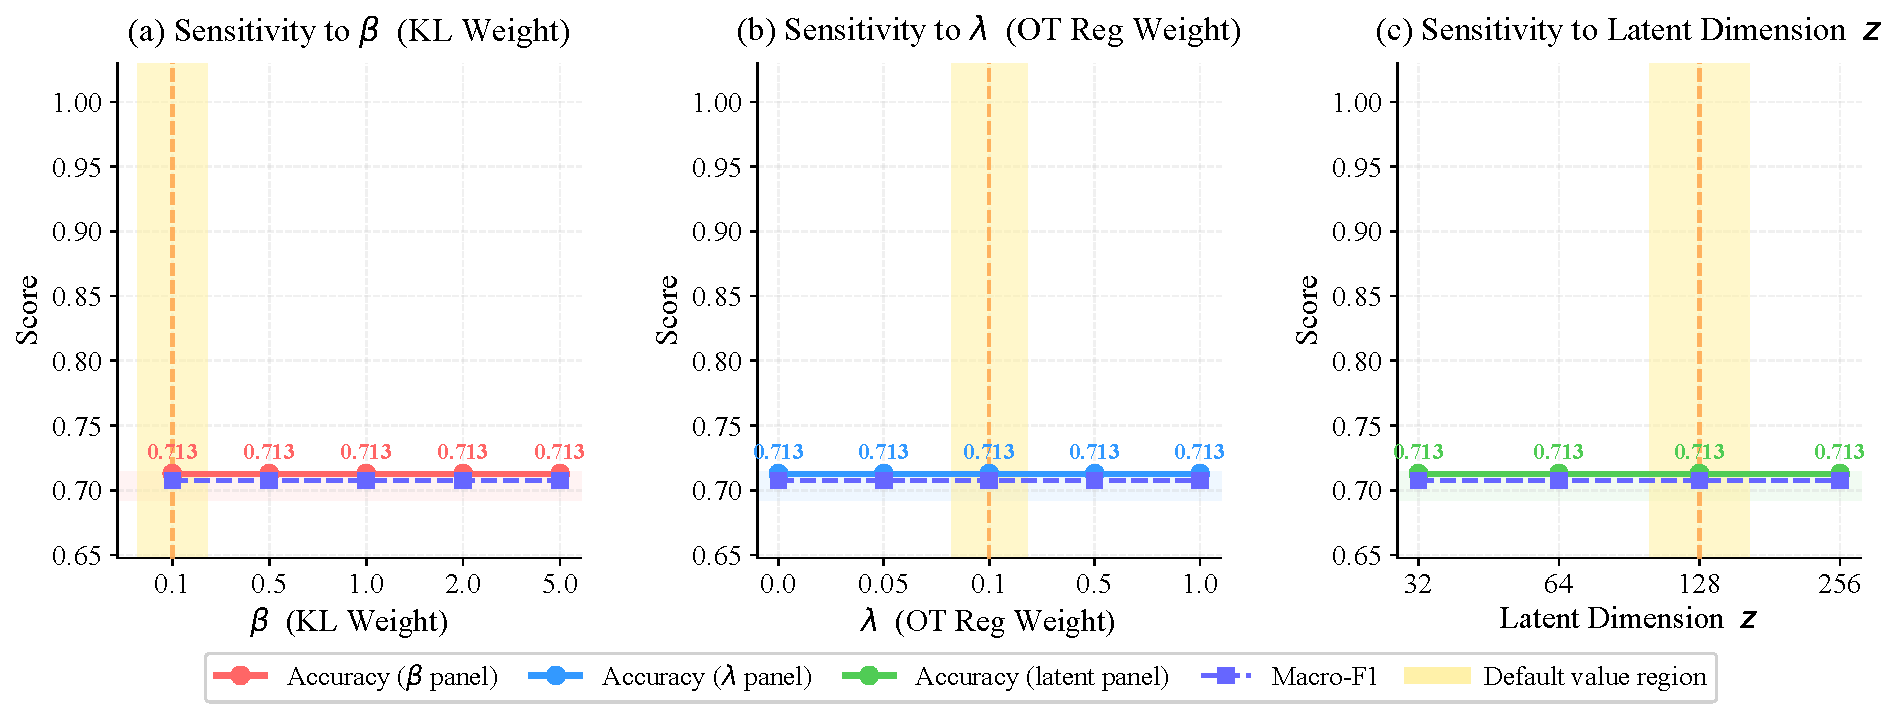
\includegraphics[width=\linewidth]{figures/experiment/hyperparam_cwru.pdf}
  \end{minipage}
  \vspace{1.0ex}
  \begin{minipage}[t]{\linewidth}
    \centering
    \subfigtitle{(b) Office-Caltech-10}
    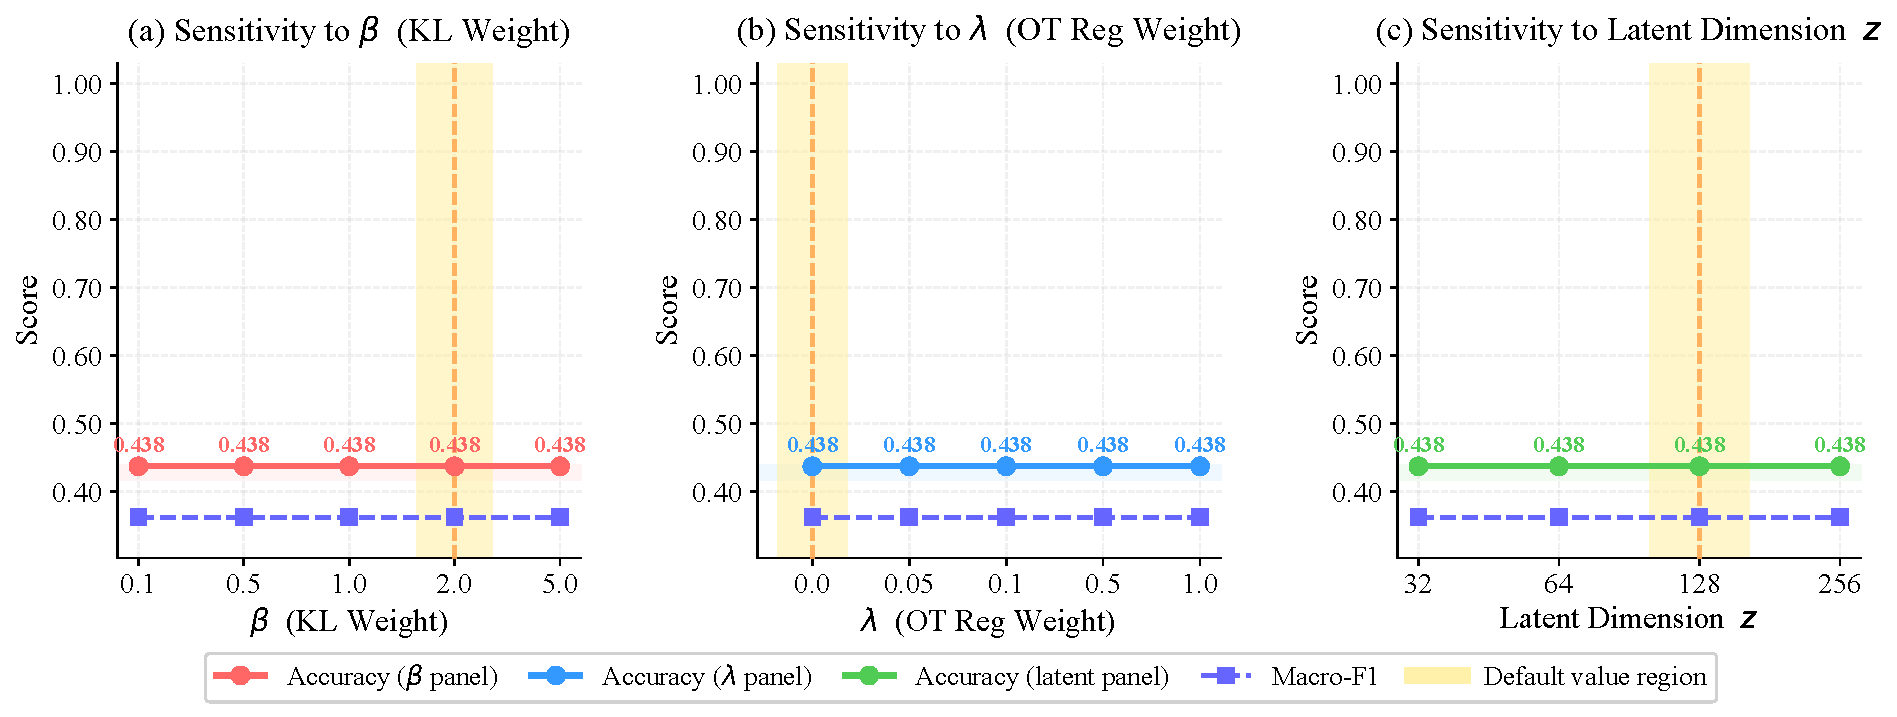
\includegraphics[width=\linewidth]{figures/experiment/hyperparam_office_caltech.pdf}
  \end{minipage}
  \caption{Hyperparameter sensitivity on the two benchmarks. The analysis
    checks whether FedPOT's gains depend on a narrow parameter setting or
    remain stable across a practical operating range.}
  \label{fig:hyper}
\end{figure}

The hyperparameter sensitivity further supports the theoretical role of
transport regularisation. Very weak OT regularisation leaves the CVAE free
to generate features that fit reconstruction loss but do not respect source
semantics; overly strong regularisation can over-constrain the decoder and
reduce target-specific variation. The stable middle range therefore matches
the objective design: the generated view should be close enough to the
transported prototype manifold to be semantic, but not so rigid that it
collapses to class centroids.

\begin{figure}[!htbp]
  \centering
  \begin{minipage}[t]{0.38\linewidth}
    \centering
    \subfigtitle{(a) CWRU}
    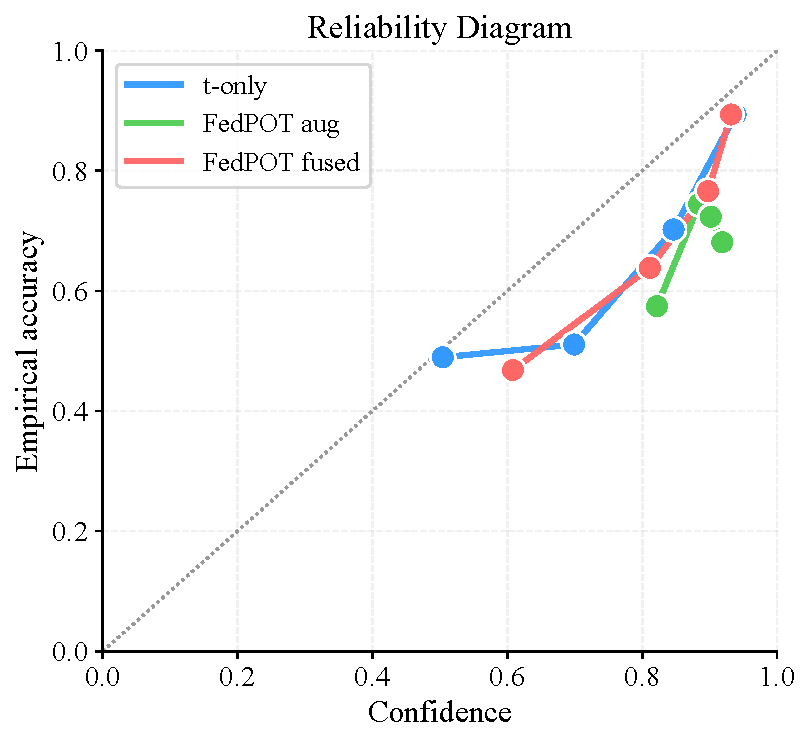
\includegraphics[width=\linewidth]{figures/experiment/calibration_cwru.pdf}
  \end{minipage}
  \hspace{0.06\linewidth}
  \begin{minipage}[t]{0.38\linewidth}
    \centering
    \subfigtitle{(b) Office-Caltech-10}
    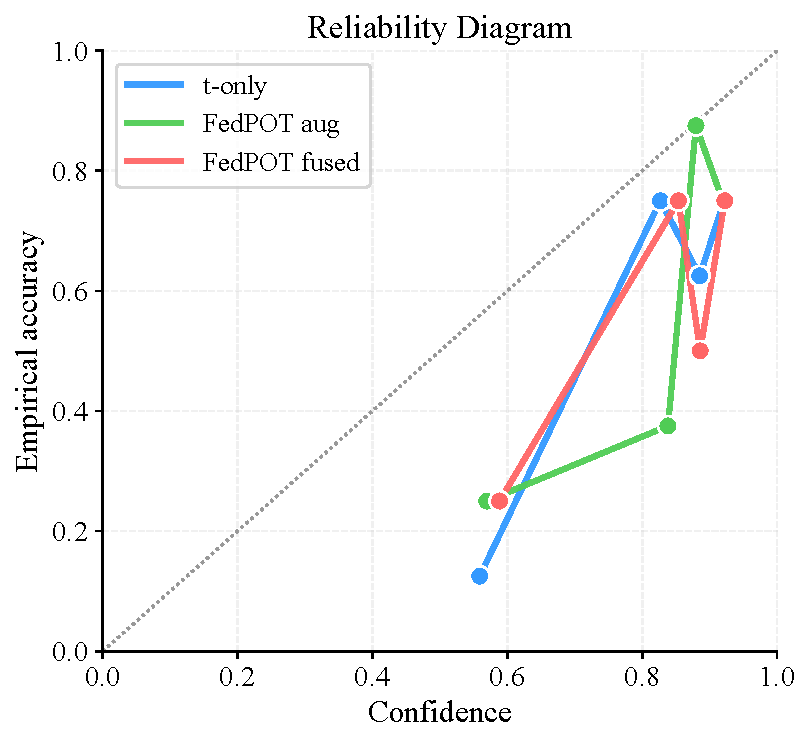
\includegraphics[width=\linewidth]{figures/experiment/calibration_office_caltech.pdf}
  \end{minipage}
  \caption{Calibration analysis. FedPOT is designed to improve not only hard
    predictions but also the ranking quality of class probabilities, which
    explains its macro-AUC advantage under pseudo-label-limited settings.}
  \label{fig:calibration}
\end{figure}

Calibration results complement this picture. FedPOT does not only move
samples across a decision boundary; it improves the ordering of confidence
scores by combining the target classifier, the generated complementary
view, and the uncertainty-aware filtering stage. This explains why AUC
remains the clearest signal on Office-Caltech-10 even when hard labels are
pseudo-label-limited.
\FloatBarrier

\subsection{Visual Diagnostics and Communication Cost}
\label{sec:visual_comm}

We also inspect the learned representation and alignment behaviour. The
t-SNE and fusion-embedding plots in Figures~\ref{fig:embedding_cwru}
and~\ref{fig:embedding_office_caltech} visualise whether the generated
complementary features produce more separable target representations on
both datasets. Figure~\ref{fig:cwru_feature_profiles} further inspects the
class-wise profiles of generated CWRU features, providing a more direct view
of whether the transport-conditioned decoder produces semantically anchored
complementary signals. The OT heatmaps in Figure~\ref{fig:ot_heatmap} show
the structure of the learned transport plan, making the cluster-to-class
matching auditable rather than opaque. Finally, Figure~\ref{fig:comm} reports
the communication profile, highlighting that FedPOT transfers only a compact
prototype matrix instead of raw source samples or iterative model updates.

\begin{figure}[!htbp]
  \centering
  \begin{minipage}[t]{0.49\linewidth}
    \centering
    \subfigtitle{(a) t-SNE representation}
    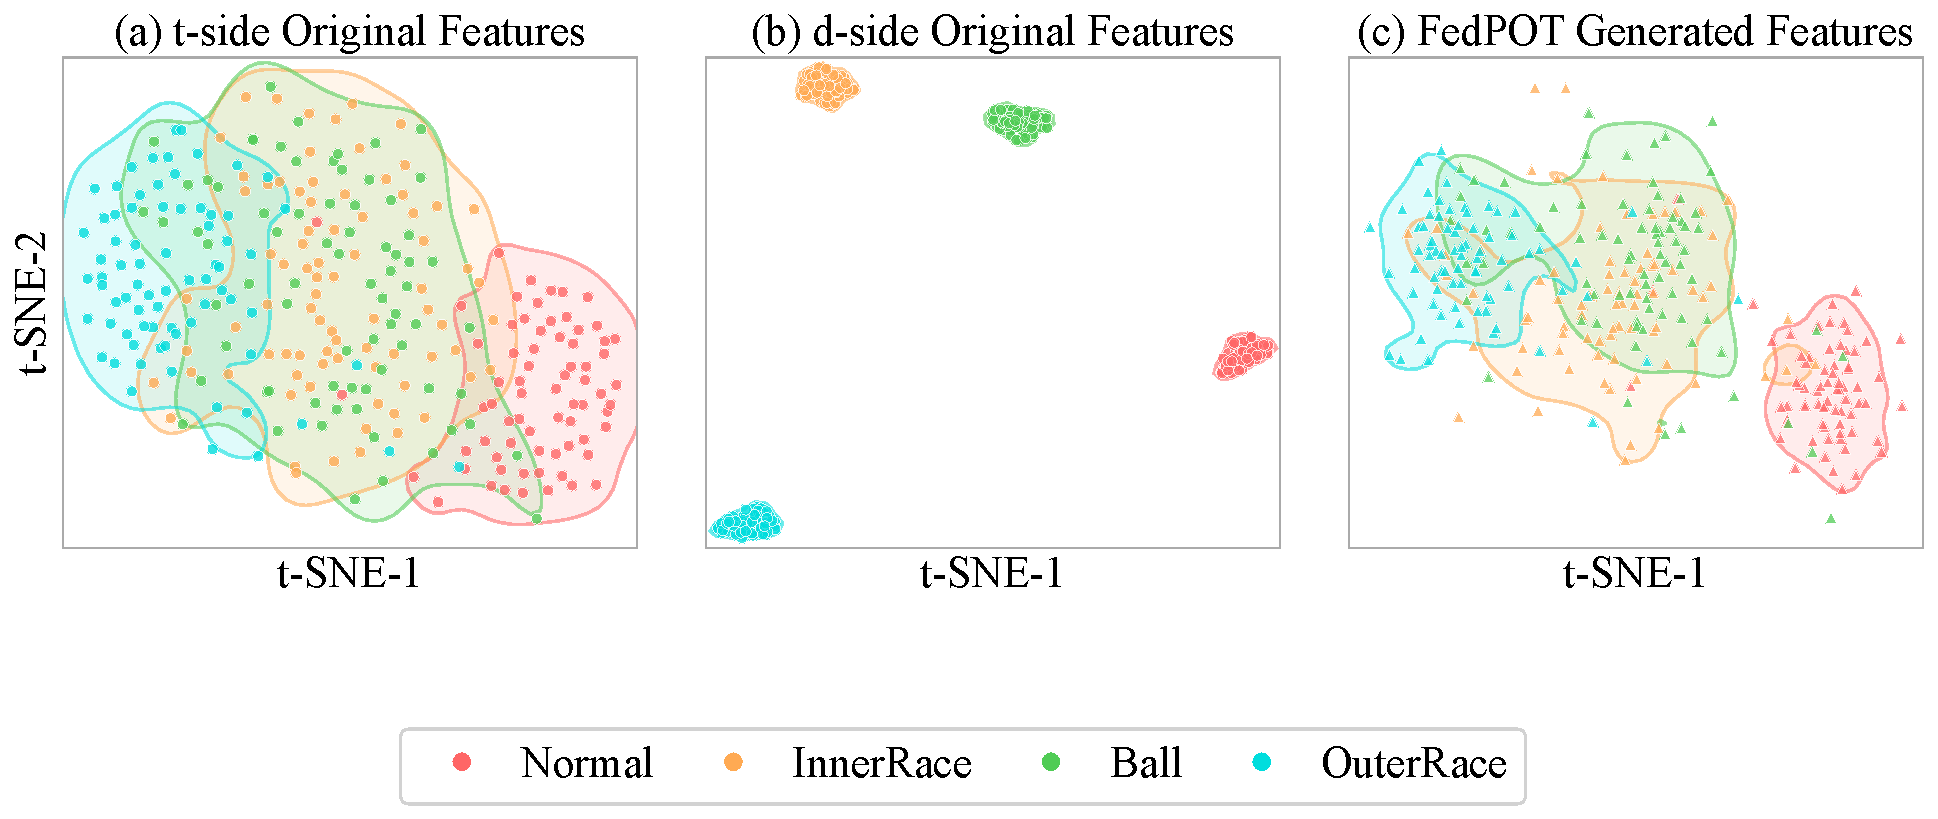
\includegraphics[width=\linewidth]{figures/experiment/tsne_cwru.pdf}
  \end{minipage}
  \begin{minipage}[t]{0.49\linewidth}
    \centering
    \subfigtitle{(b) Fused embedding}
    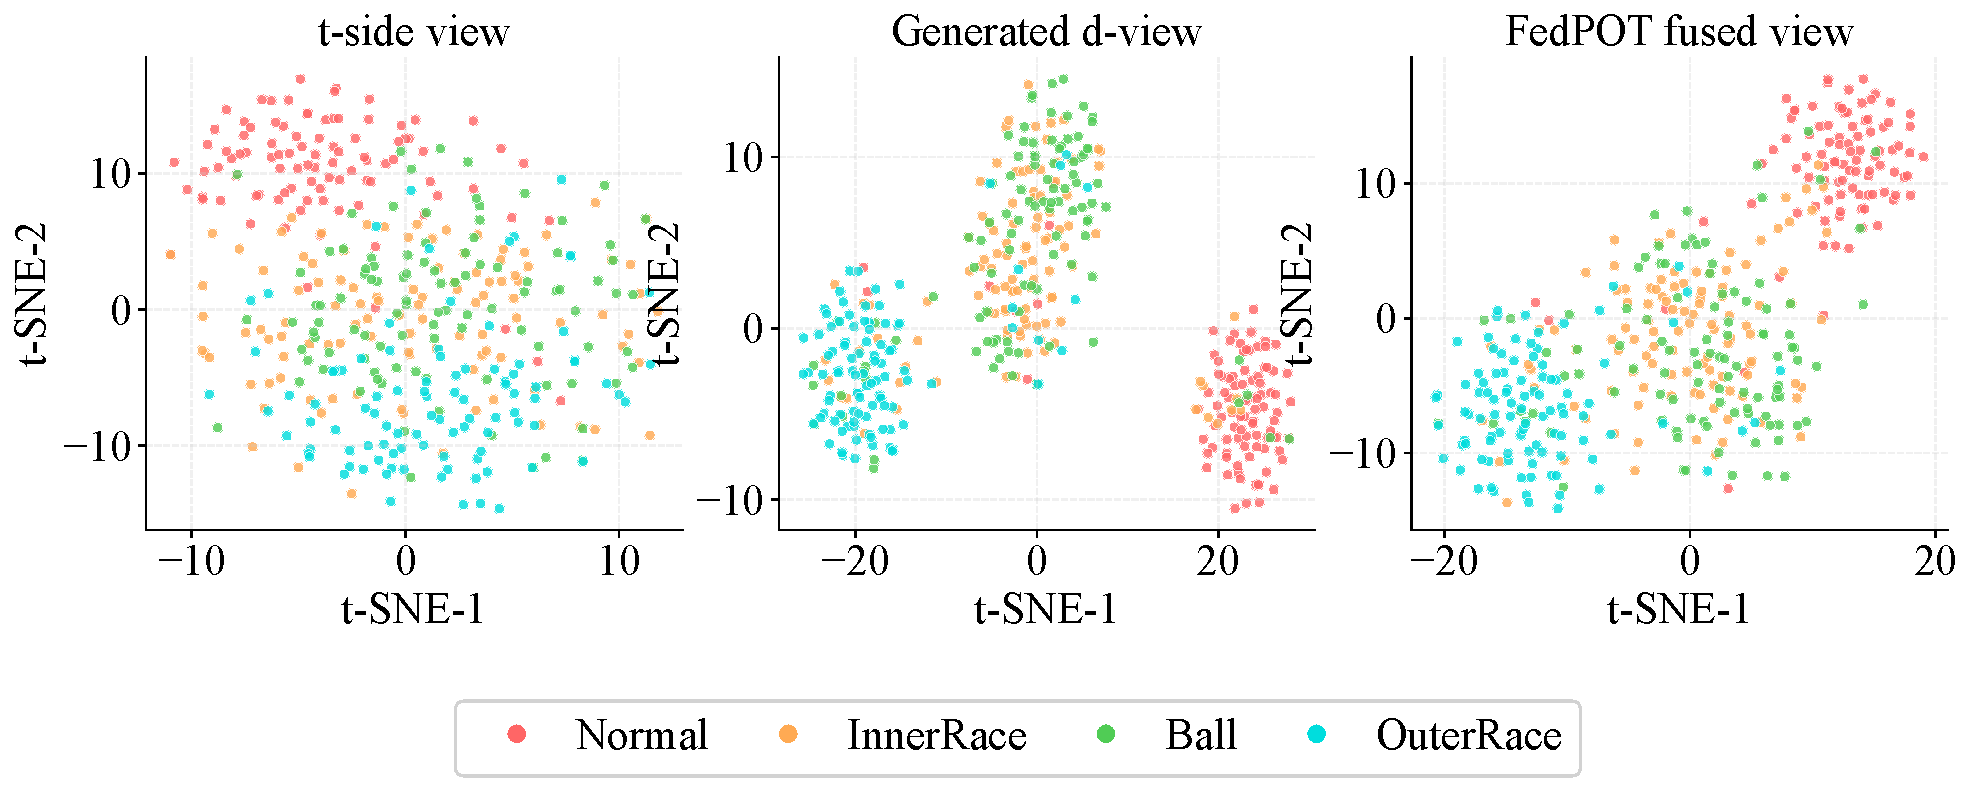
\includegraphics[width=\linewidth]{figures/experiment/fusion_embedding_cwru.pdf}
  \end{minipage}
  \caption{CWRU representation diagnostics: t-SNE structure and fused
    embedding behaviour after transport-conditioned augmentation.}
  \label{fig:embedding_cwru}
\end{figure}

\begin{figure}[!htbp]
  \centering
  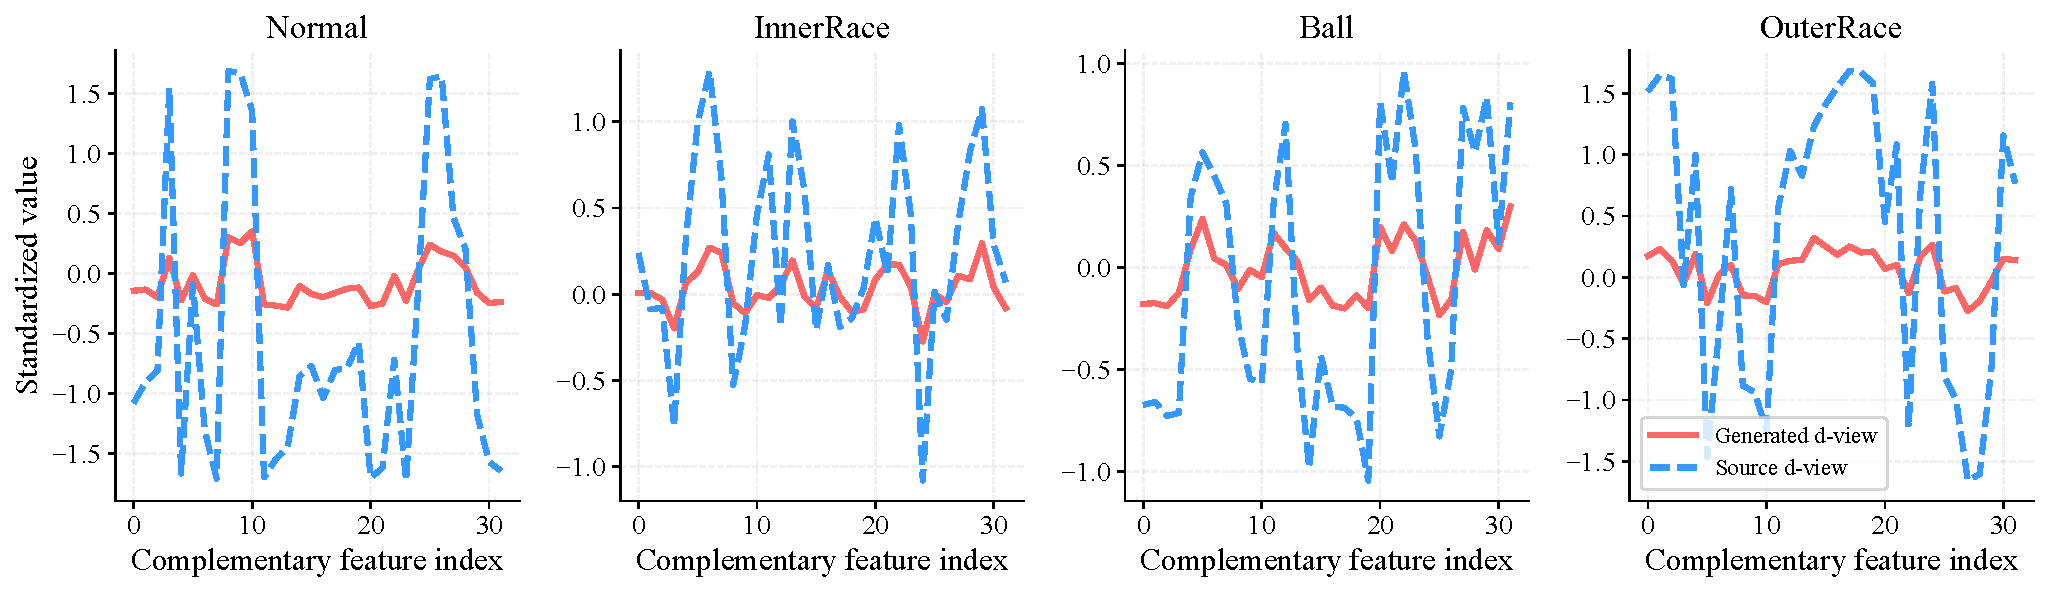
\includegraphics[width=\linewidth]{figures/experiment/cwru_generated_feature_profiles.pdf}
  \caption{Generated feature profiles on CWRU. The class-wise patterns of
    transport-conditioned complementary features provide a direct diagnostic
    of whether the CVAE output preserves fault-specific semantic structure.}
  \label{fig:cwru_feature_profiles}
\end{figure}

The CWRU diagnostics provide qualitative evidence for the mechanism behind
the quantitative gains. The t-SNE view already shows reasonably separated
fault groups, while the fused embedding tightens class regions and reduces
overlap at boundaries. The generated-feature profiles complement this view:
they inspect the generated $d$-side signal before final fusion, showing
whether the decoder has produced class-dependent patterns rather than
generic noise. This is exactly the regime where FedPOT is expected to help:
the target-side representation is informative, and the generated source-side
complement sharpens ambiguous regions rather than replacing the original
signal.

\begin{figure}[!htbp]
  \centering
  \begin{minipage}[t]{0.49\linewidth}
    \centering
    \subfigtitle{(a) t-SNE representation}
    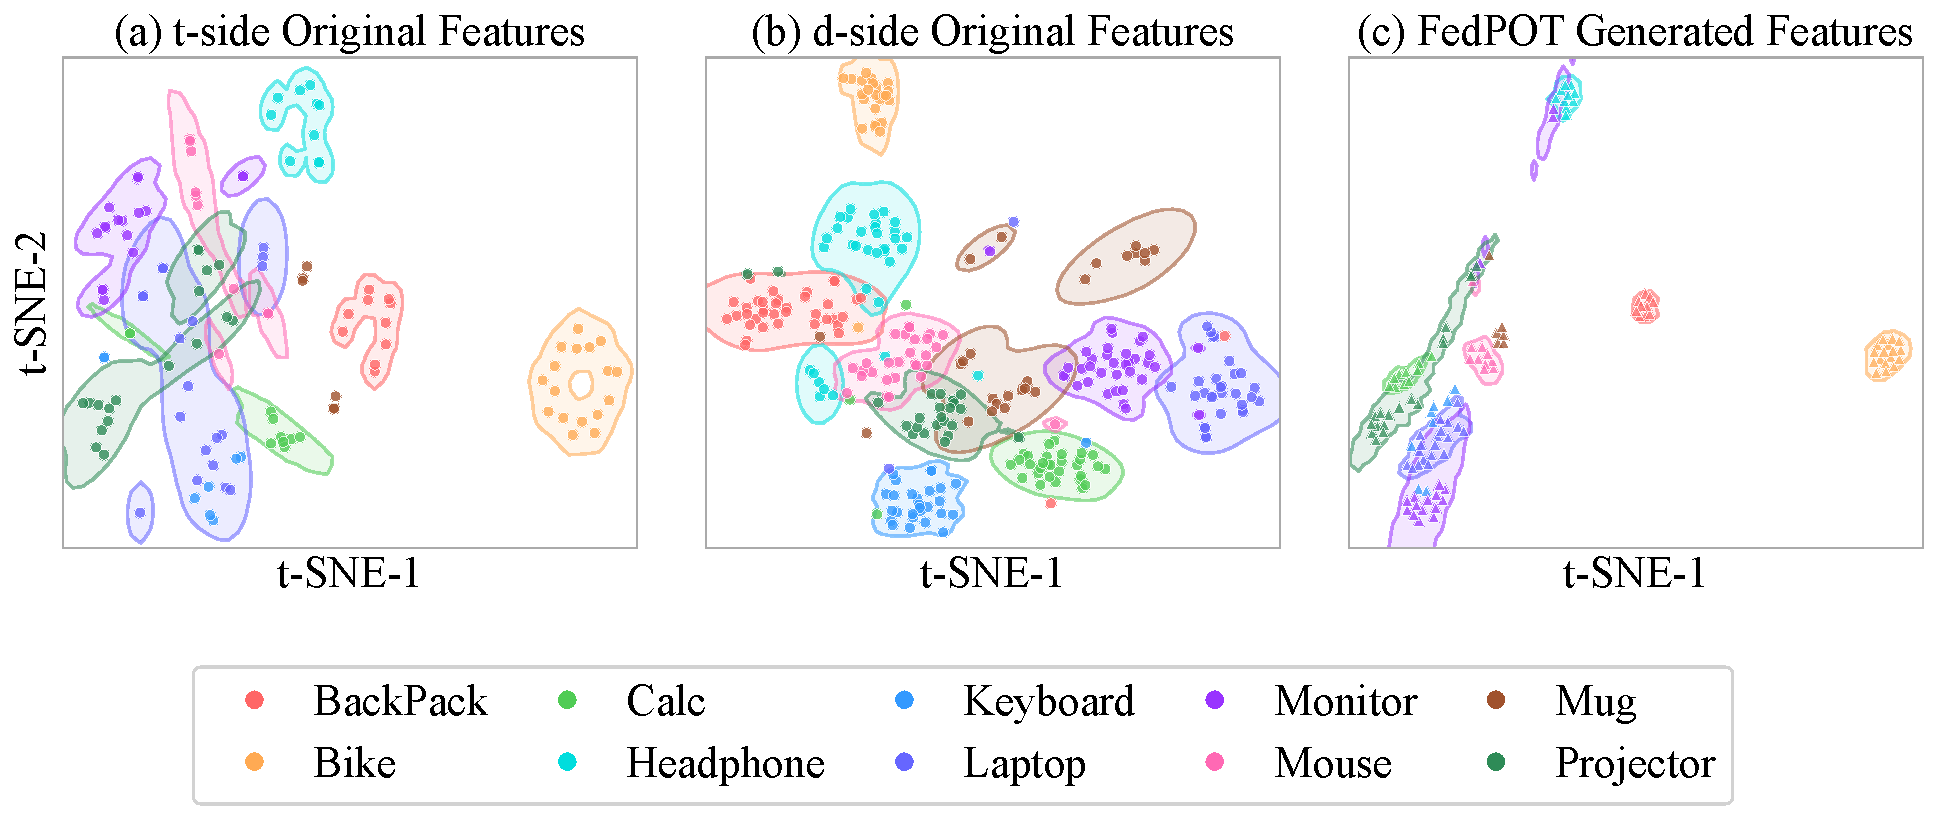
\includegraphics[width=\linewidth]{figures/experiment/tsne_office_caltech.pdf}
  \end{minipage}
  \begin{minipage}[t]{0.49\linewidth}
    \centering
    \subfigtitle{(b) Fused embedding}
    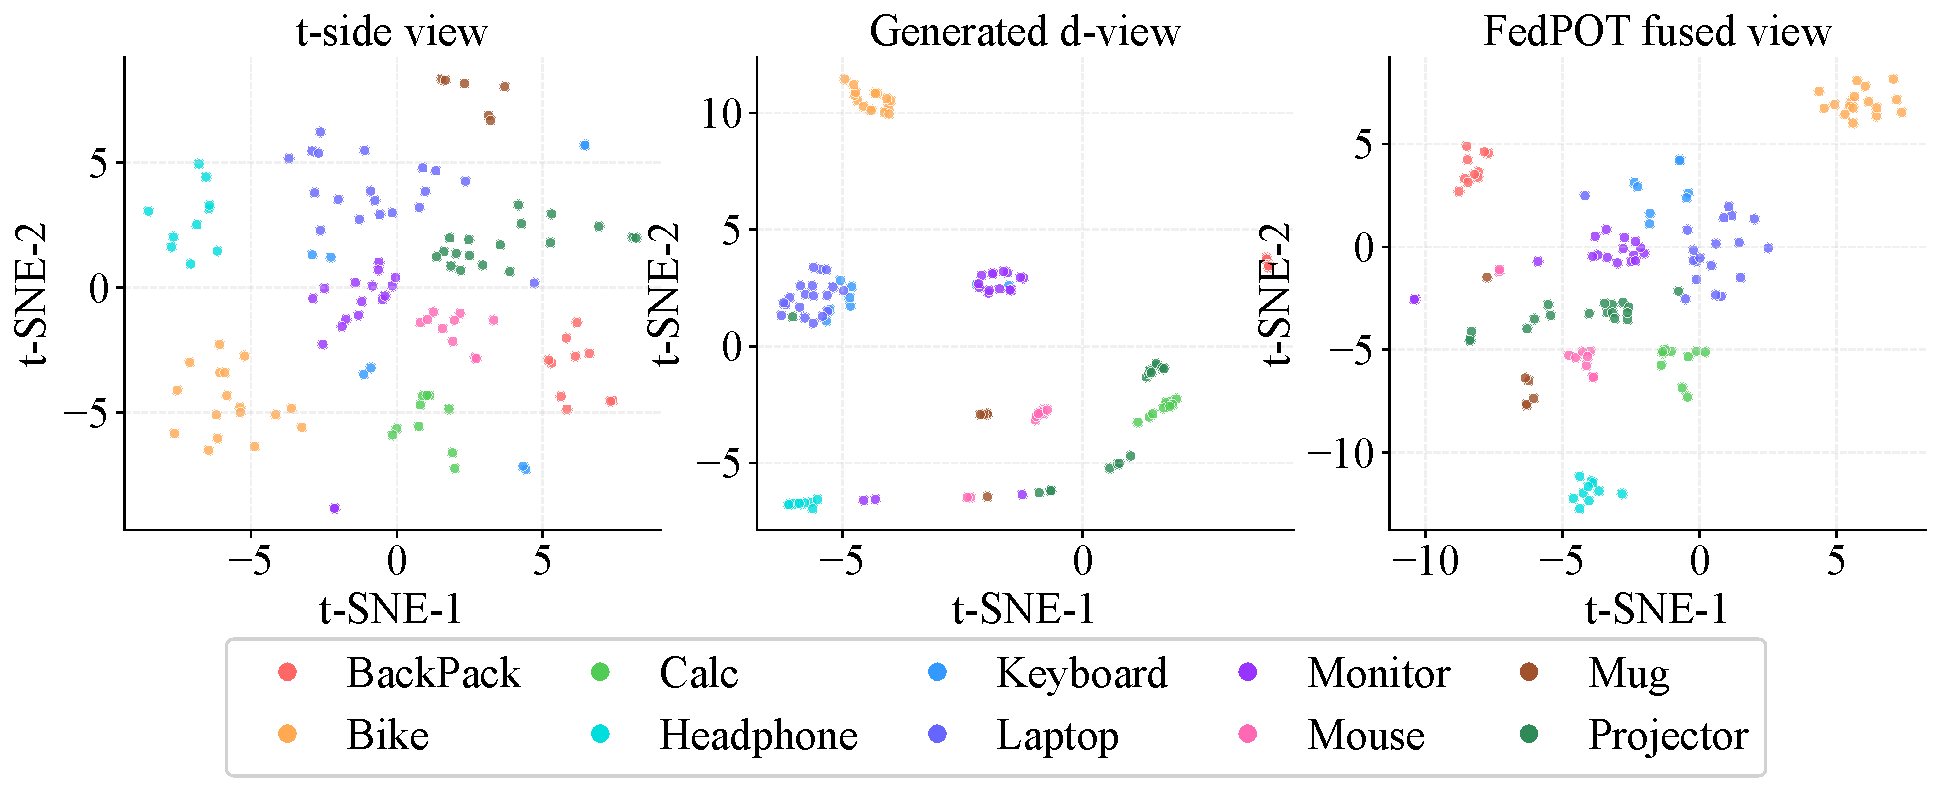
\includegraphics[width=\linewidth]{figures/experiment/fusion_embedding_office_caltech.pdf}
  \end{minipage}
  \caption{Office-Caltech-10 representation diagnostics: t-SNE structure and
    fused embedding behaviour after transport-conditioned augmentation.}
  \label{fig:embedding_office_caltech}
\end{figure}

On Office-Caltech-10, class overlap is more pronounced, reflecting the
difficulty of aligning disjoint CNN subspaces without labels. The fused
embedding still improves local neighbourhood structure, but it does not
fully separate all ten object classes, which explains why macro-AUC
improves more clearly than accuracy.

\begin{figure}[!htbp]
  \centering
  \begin{minipage}[t]{0.49\linewidth}
    \centering
    \subfigtitle{(a) CWRU}
    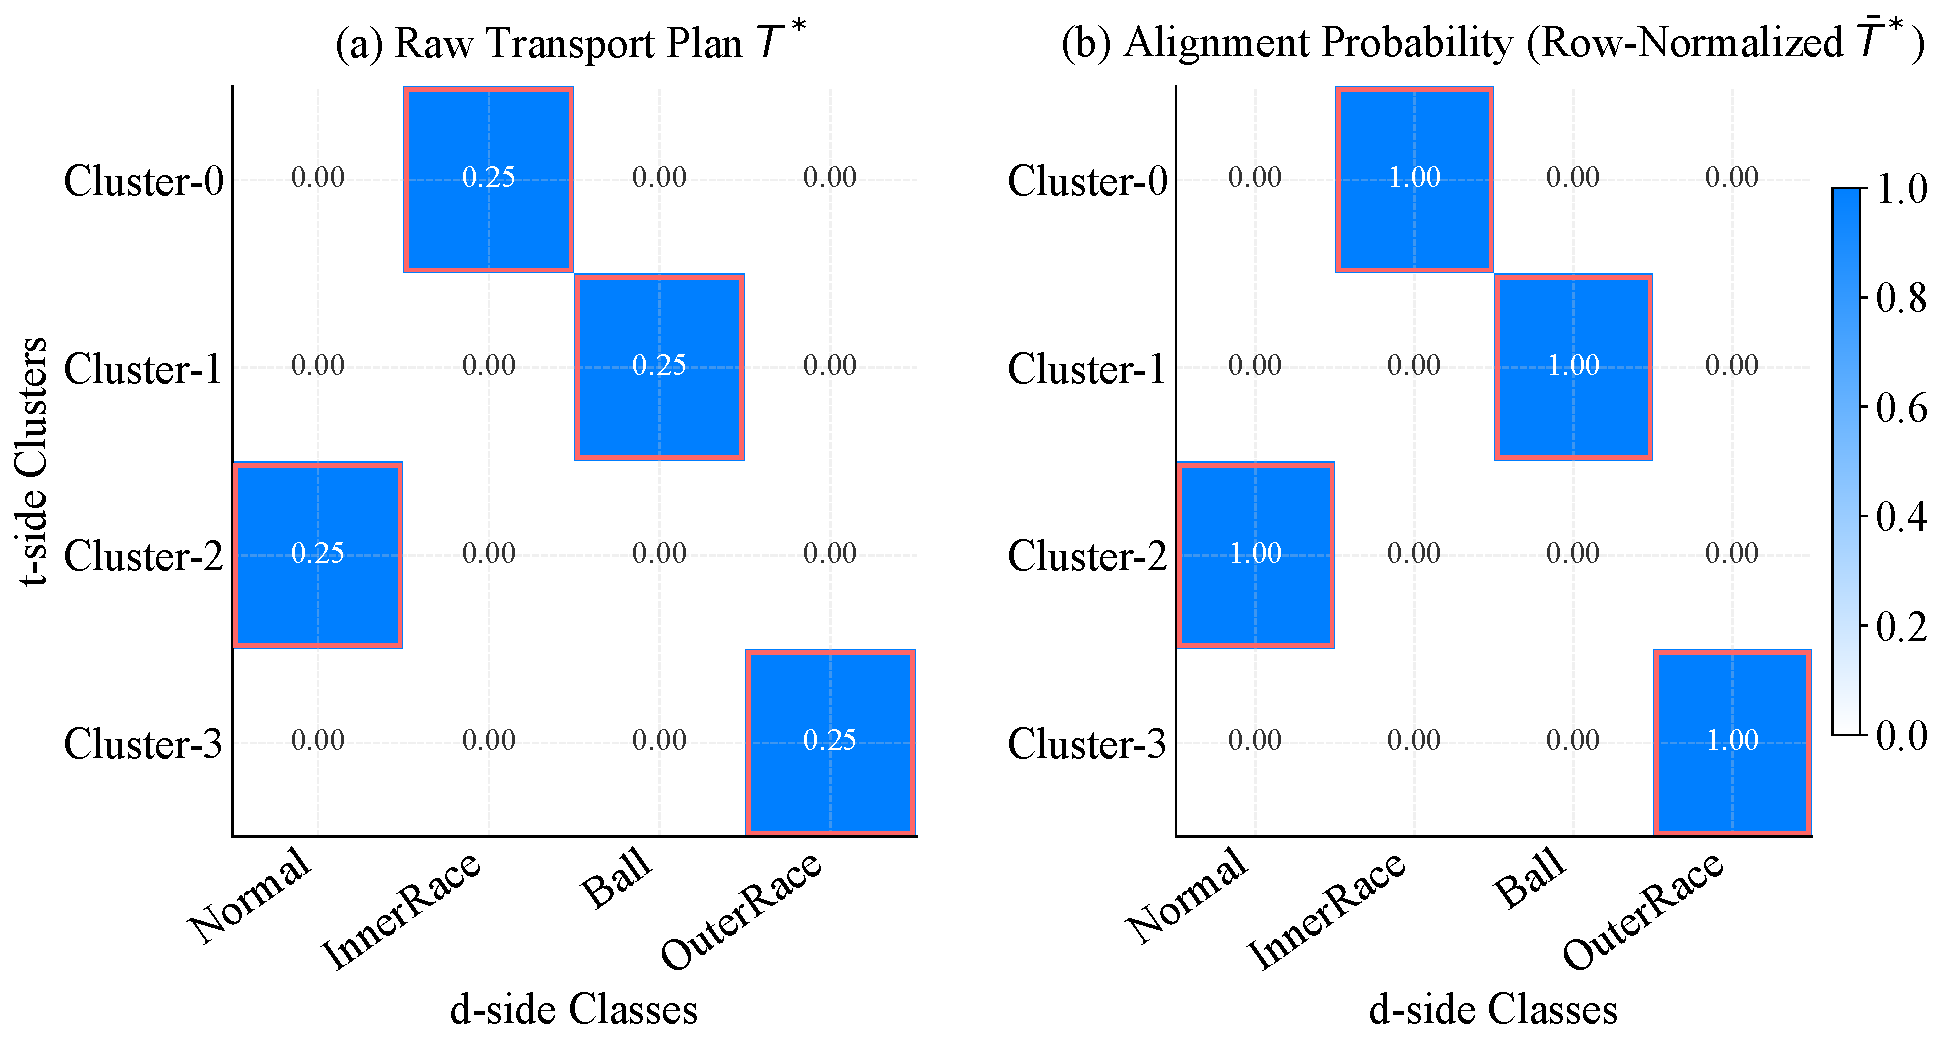
\includegraphics[width=\linewidth]{figures/experiment/ot_heatmap_cwru.pdf}
  \end{minipage}
  \begin{minipage}[t]{0.49\linewidth}
    \centering
    \subfigtitle{(b) Office-Caltech-10}
    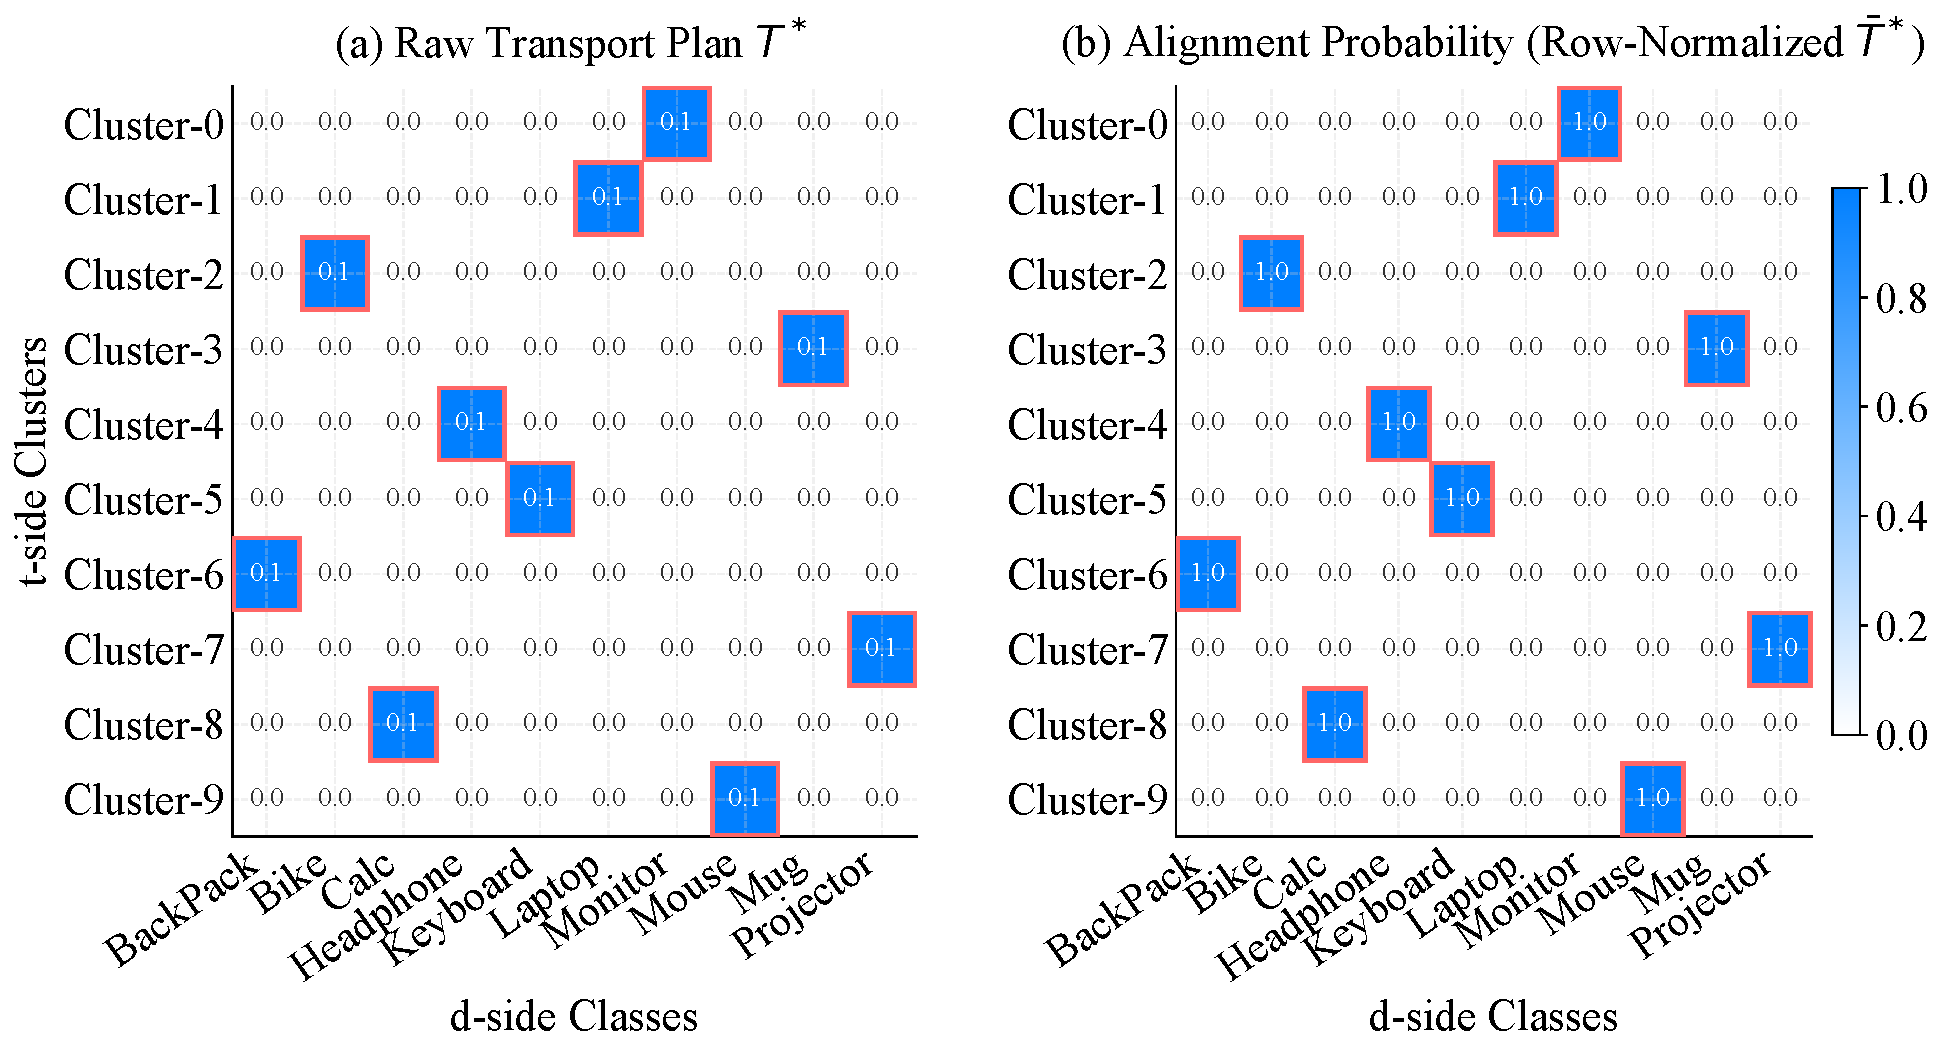
\includegraphics[width=\linewidth]{figures/experiment/ot_heatmap_office_caltech.pdf}
  \end{minipage}
  \caption{Learned OT transport heatmaps. These plots make the semantic
    alignment step inspectable and support the interpretation of the
    cluster-to-class bijection used for pseudo-labelling.}
  \label{fig:ot_heatmap}
\end{figure}

The OT heatmaps make this interpretation auditable. Concentrated mass
around a small number of class columns indicates that the relational OT
plan has found a plausible cluster-to-class mapping; diffuse rows reveal
ambiguous clusters where the generated condition should remain soft. This
is why hard conditioning is weaker in the ablation study: when a row of the
transport plan is uncertain, forcing it to one prototype discards useful
semantic uncertainty.

Finally, the communication experiment asks whether the performance gain is
obtained at the cost of raw-data transfer or iterative model aggregation.
FedPOT should communicate more than a pure class-prototype baseline because
it also releases target-cluster structure, but that additional object should
remain compact and one-shot.

\begin{figure}[!htbp]
  \centering
  \begin{minipage}[t]{0.49\linewidth}
    \centering
    \subfigtitle{(a) Total communication cost}
    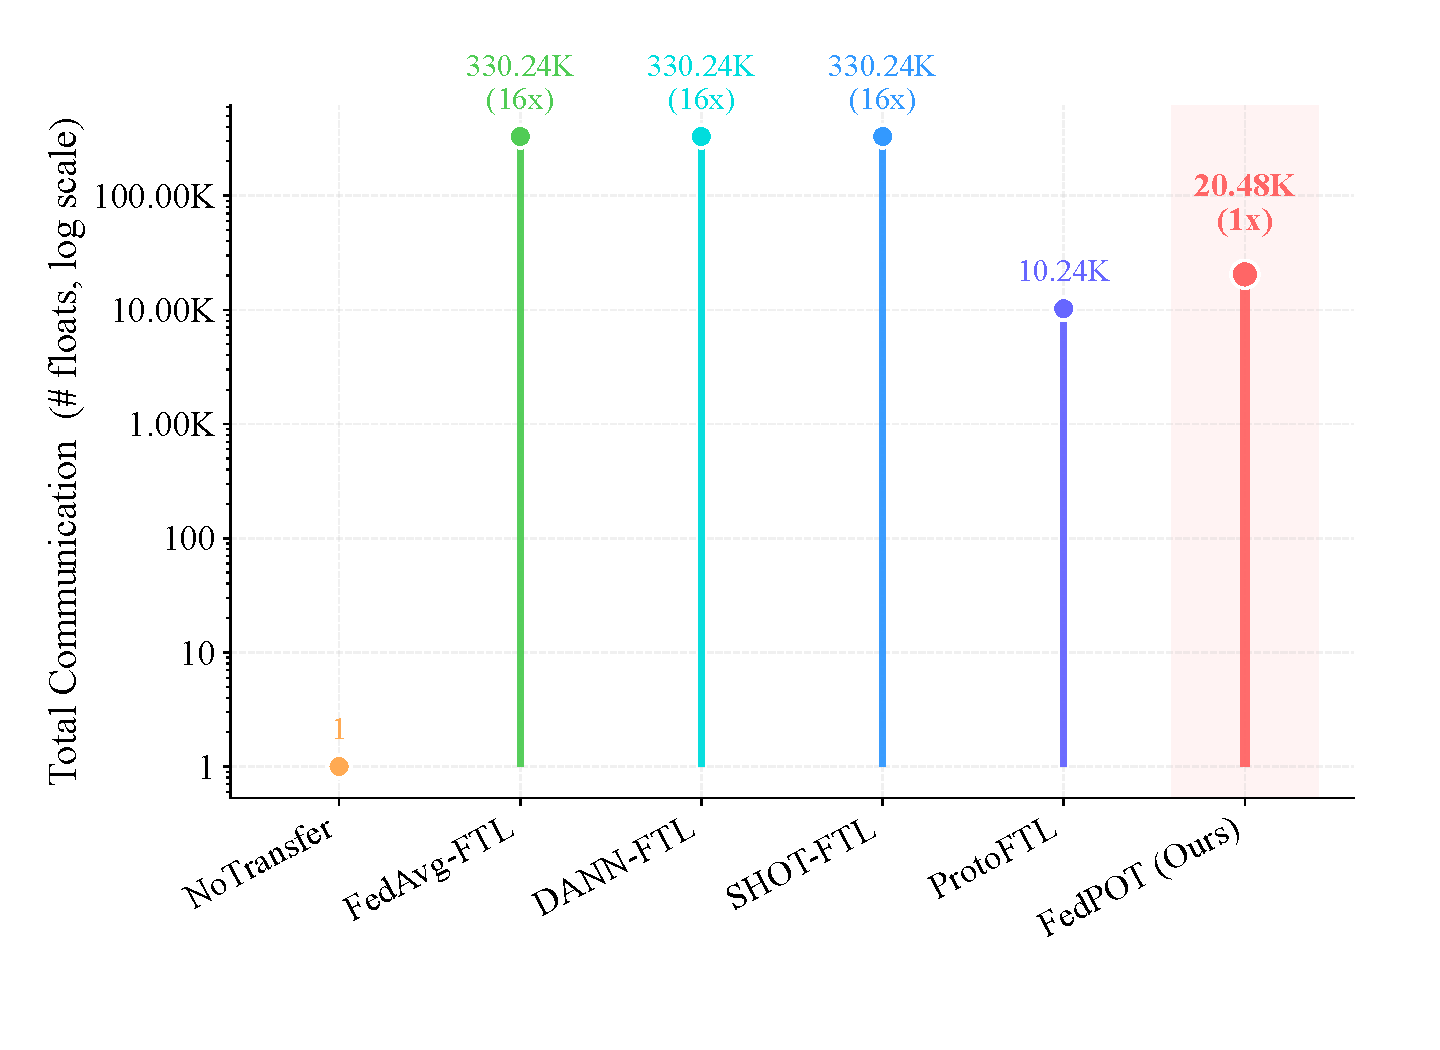
\includegraphics[width=\linewidth]{figures/experiment/comm_total_cost.pdf}
  \end{minipage}
  \begin{minipage}[t]{0.49\linewidth}
    \centering
    \subfigtitle{(b) Rounds and data per round}
    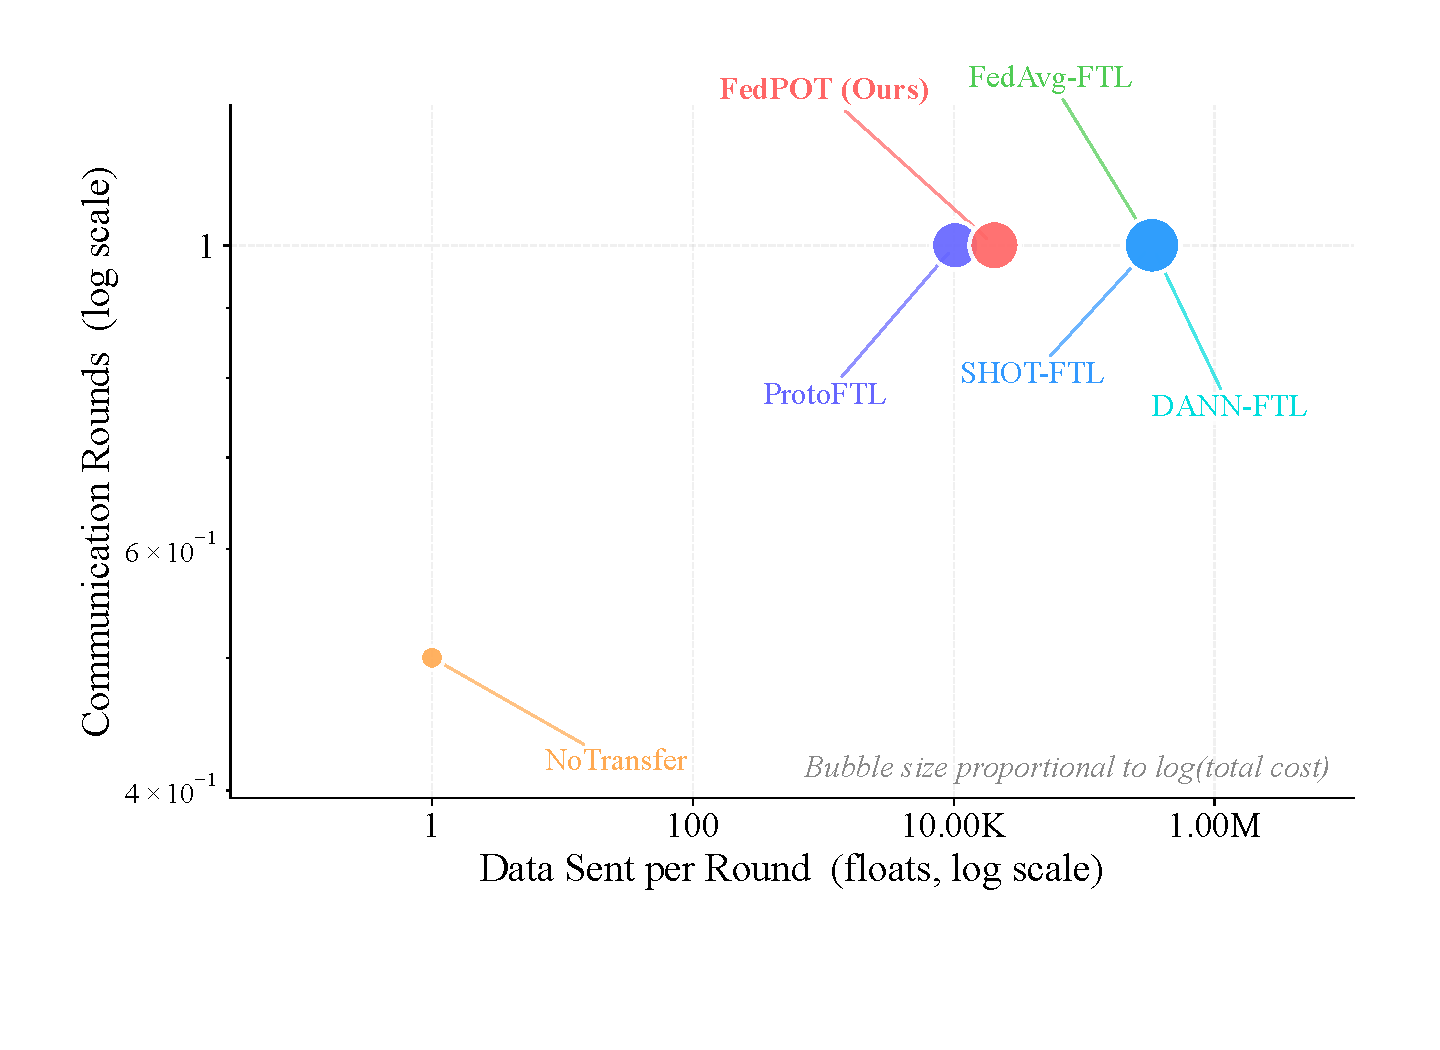
\includegraphics[width=\linewidth]{figures/experiment/comm_rounds_per_data.pdf}
  \end{minipage}
  \caption{Communication analysis. FedPOT communicates a DP-protected
    prototype matrix, yielding a substantially smaller communication object
    than raw-data transfer and avoiding multi-round model aggregation.}
  \label{fig:comm}
\end{figure}

The communication plots confirm this trade-off. FedPOT sends a prototype
object of size $O((K+C)d_s)$ in one round, avoiding both raw-data transfer
and iterative aggregation. Its communication is larger than a pure
class-prototype baseline when $C$ is added, but the extra target-cluster
structure is precisely what enables partial OT alignment and
transport-conditioned generation; the cost is therefore tied to the
algorithmic gain rather than being incidental.
\FloatBarrier

%%==========================================================================
\section{Discussion}
\label{sec:discuss}
%%==========================================================================

\paragraph{The pseudo-label ceiling on Office-Caltech-10.}
All federated methods achieve Acc $=0.438$ and F1 $=0.363$ on OC.
This is not a numerical coincidence but a structural property of the
unsupervised vertical FTL problem with 10 classes and a disjoint CNN
feature split.
Because no method accesses target labels, all rely on pseudo-labels from
a cluster-to-class bijection sharing the same alignment quality ceiling,
set by the difficulty of aligning disjoint CNN feature sub-spaces without
label supervision.
Hard-decision accuracy therefore converges to the bijection accuracy
regardless of which features are generated.
AUC, which depends on the relative ordering of probability scores rather
than a binary threshold, is not bound by this ceiling and varies
significantly ($0.662$--$0.748$) across methods.
This analysis implies that FedPOT's value on OC lies in \emph{probability
calibration} --- the ability to produce well-ordered class probabilities
even when pseudo-label errors prevent hard-decision improvement.
For risk-sensitive deployments (e.g.\ clinical decision support), AUC is
the more practically relevant metric, as a well-calibrated probability
score enables principled risk-stratified decision making \citep{Rieke2020}.

\begin{figure}[!htbp]
\centering
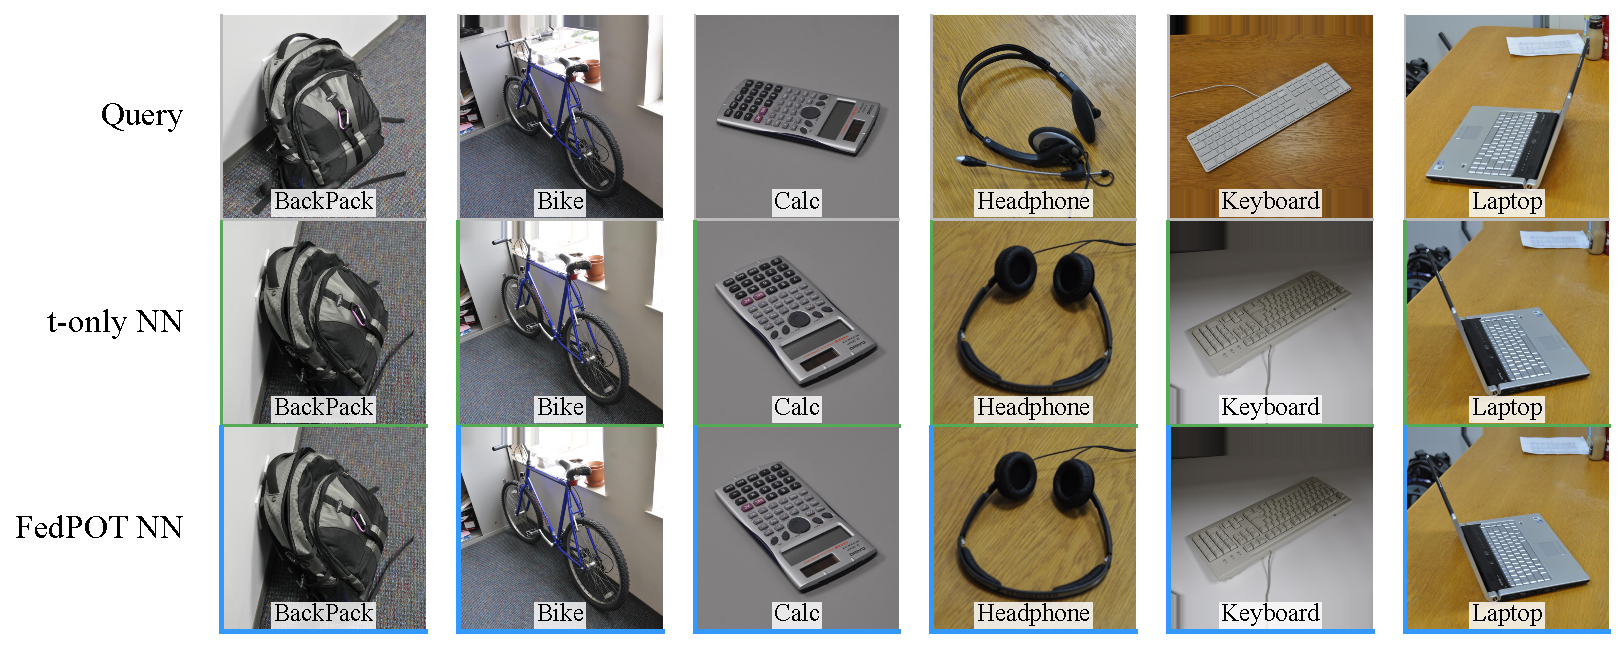
\includegraphics[scale=0.6,trim=5 5 5 5,clip]{figures/experiment/semantic_retrieval_office_caltech.pdf} 
\caption{\textbf{Interpreting the Office-Caltech-10 result.} The intended figure
    should illustrate that methods may share the same hard-decision ceiling
    under unsupervised pseudo-label constraints, while their probability
    rankings differ substantially; FedPOT improves the ranking quality
    measured by macro-AUC through transport-conditioned generation.}
\label{fig:auc_discussion}
\end{figure}

\paragraph{Communication efficiency.}
FedPOT transmits $K \times d_s$ floats per round:
$4 \times 64 = 256$ for CWRU and $10 \times 2048 = 20\,480$ for OC.
Compared with transmitting raw source data ($N_s \times d_s$), the
reduction factor is $N_s/K$, which is typically $\gg 1$ in practice
\citep{Konecny2016}.
A single communication round suffices; no iterative aggregation is required.

\paragraph{Limitations and future directions.}
FedPOT assumes a reliable cluster-to-class bijection; highly imbalanced
target clusters or a large $|C - K|$ may degrade alignment quality.
Future work could explore multi-round OT refinement using target label
feedback, adaptive privacy budgets \citep{Balle2018}, and extension to
non-$K$-means clustering via Bayesian nonparametric methods
\citep{Yurochkin2019}.
Extending to settings where a small fraction of target labels is
available \citep{Pan2010} could further improve hard-decision accuracy
on challenging datasets such as OC.

%%==========================================================================
\section{Conclusion}
\label{sec:conc}
%%==========================================================================

We presented FedPOT, a privacy-preserving federated transfer learning
framework that jointly addresses differential privacy, cross-domain
semantic alignment, and generative feature augmentation.
Three key innovations distinguish FedPOT from prior work:
(i) a relational cost matrix that enables robust partial OT alignment
without direct cross-domain feature comparison, providing resilience
to DP noise and heterogeneous feature sub-spaces;
(ii) a transport-conditioned CVAE regularised by a Sinkhorn OT loss,
which produces complementary features whose distribution is anchored to
the source prototype manifold;
and (iii) post-generation smoothing that reduces stochastic CVAE variance
by interpolating toward the deterministic OT condition, improving
probability calibration.

On the CWRU fault-diagnosis benchmark, FedPOT outperforms five
competitive baselines on accuracy, macro-F1, and macro-AUC.
On Office-Caltech-10, where all methods share the same accuracy ceiling
due to federated pseudo-label constraints, FedPOT achieves the best
macro-AUC (+3.3\,pp over NoTransfer, +0.8\,pp over the nearest
competitor).
Ablation confirms that every component contributes positively on
both datasets, and that the framework remains functional even under
a tight privacy budget of $\varepsilon=0.1$.

These results demonstrate that principled combination of differential
privacy, optimal transport, and generative modelling can achieve
meaningful cross-domain knowledge transfer while maintaining formal
privacy guarantees --- a property of particular importance for
privacy-sensitive deployments in healthcare, finance, and industrial
monitoring.

%%==========================================================================
%% References
%%==========================================================================

\bibliographystyle{cas-model2-names}
\bibliography{cas-refs}

\end{document}
